\documentclass[english]{scrartcl}

\usepackage{fullpage}
\usepackage{amstext,amssymb,amsmath,amsthm}
\usepackage{graphicx,subfigure}
\usepackage{multirow}
\usepackage{url}
\usepackage{hyperref}
\usepackage{color}

\graphicspath{{.}{pics/}}

%\newtheorem{theorem}{Theorem}[section]
%\newtheorem{proposition}[theorem]{Proposition}


\title{Composite Bayesian inference}
\date{}
\author{Alexis Roche\thanks{\url{alexis.roche@centraliens.net}}}

%\newcommand{\fix}{\marginpar{FIX}}
%\newcommand{\new}{\marginpar{NEW}}
%\newcommand{\matphi}{\boldsymbol{\Phi}} 
%\def\x{{\mathbf{x}}}
%\def\z{{\mathbf{z}}}
%\def\u{{\mathbf{u}}}
%\def\p{{\bar{\mathbf{p}}}}
%\def\q{{\bar{\mathbf{q}}}}



\begin{document}

\maketitle

\begin{abstract}
This note revisits the concept of composite likelihood from the perspective of probabilistic inference, and advocates a machine learning approach to tune the associated ``weights'', which stems naturally from a connection with the maximum entropy principle: the predictive distribution that maximizes conditional entropy relative to a given prior and subject to multiple mean log-likelihood inequality constraints is, up to a normalizing factor, the prior multiplied by a particular composite likelihood function, hence providing a ``composite'' extension of Bayes rule. We argue that composite Bayesian inference is a middle way between generative and discriminative approaches to statistical inference, which can be powerful in shallow learning and transfer learning problems.
\end{abstract}


\section{Introduction}
\label{sec:intro}

Frequentist and Bayesian inference are based on the concept of likelihood, which relies on the existence of a statistical data-generating model that is both experimentally plausible and computationally tractable. Because this is challenging for complex data, other paradigms are commonly used in applied science: deliberately misspecified generative models, as in quasi-likelihood methods \cite{White-82,Walker-13} or na\"ive Bayes \cite{Ng-01}; minimum description length \cite{Grunwald-07}; and, last but not least, discriminative models\footnote{A {\em discriminative} model is a parametric family that describes the conditional distribution of an unobserved variable of interest given an observable variable, in contrast with a {\em generative} model, which describes the conditional distribution of an observable variable given an unobserved variable.}, which currently dominate the field of artificial intelligence and typically require heavy supervised learning -- these include classical techniques such as maximum entropy classifiers \cite{BergerA-96}, support vector machines \cite{Vapnik-00}, Gaussian processes \cite{Rasmussen-06}, as well as most deep learning techniques \cite{Lecun-15,Goodfellow-16} with the exception of deep belief networks \cite{Hinton-06,Fischer-14}. 

A strong limitation of discriminative models is that they are not suitable for unsupervised learning or on-the-fly parameter estimation because they treat the data and the model parameters as {\em marginally independent}, meaning that the data conveys no information about the parameters unless the variable of interest is observed. This is illustrated in Figure~\ref{fig:graph_comparison} by the respective directed graph representations of generative and discriminative models. For the same reason, supervised learning in discriminative models is less precise than in comparable generative models, hence less effective in small training sets \cite{Ng-01}. Overall, pure discriminative models are of little use outside the context of big labeled data.

% p(x,y|theta) = p(x|y,theta)p(y|theta)

\begin{figure}[!ht]
\begin{center}
\subfigure[Generative model]{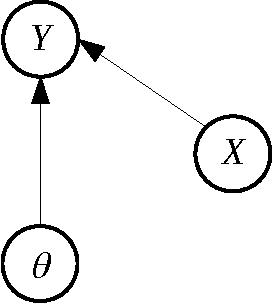
\includegraphics[width=.25\textwidth]{generative.pdf}\label{fig:generative}}
\hspace*{.2\textwidth}
\subfigure[Discriminative model]{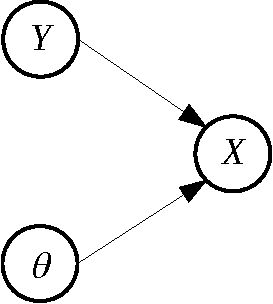
\includegraphics[width=.25\textwidth]{discriminative.pdf}\label{fig:discriminative}}
\caption{Bayesian networks representing generative and discriminative models, where $X$, $Y$ and $\theta$ respectively denote the variable of interest, the data, and the model parameters. Note the marginal independence of~$Y$ and~$\theta$ in the discriminative model.}
\label{fig:graph_comparison}
\end{center}
\end{figure}

Composite likelihood (CL, see \cite{Varin-11} and the references therein) is a semi-generative approach to statistical inference that extends the familiar notion of likelihood without requiring a full generative model. The key idea is to model an arbitrary set of low-dimensional features separately and then combine them, instead of modeling the data distribution as a whole. This may be viewed as a {\em divide and conquer} method to approximate the true but intractable likelihood. While maximum CL does not inherit the general property of maximum likelihood to yield an asymptotically minimum-variance estimator, it is consistent under mild conditions \cite{Xu-11} and may offer an excellent trade-off between computational and statistical efficiency in practice. 

In this note, CL is interpreted as a probabilistic opinion pool of ``agents'' making use of different pieces of information, or clues, extracted from the input data. Each agent acts as an isolated generative model-based statistician and expresses an opinion based on a single clue in the form of a likelihood function of the hidden variables. The agent opinions are then aggregated into a probability distribution on the hidden variables analogous to a Bayesian posterior.

We further argue that a particular log-linear opinion pool yields the best possible predictive distribution in the sense of maximum relative conditional entropy. This perspective entails a method to optimize the weights of the different agents from training data as in a typical discriminative learning scenario. 

%Something for true statisticians. Maybe we could clarify that we use the term ``Bayesian'' in the sense of ``empirical Bayesian'', implying that the parameters $\theta$ are to be estimated somehow contrary to a ``full Bayesian'' approach where they would be integrated out at inference time.


\section{Composite likelihood as opinion pooling}
\label{sec:pool}

Let $Y$ an observable multivariate random variable with sampling distribution $p(y|x)$ conditional on some unobserved variable of interest, $X\in{\cal X}$, where ${\cal X}$ is a known set. Given an experimental outcome $y$, the likelihood is the sampling distribution evaluated at $y$, seen as a function of $x$:
$$
L(x) = p(y|x)
.
$$

This requires a plausible generative model which, for complex data, may be out of reach or involve too many parameters to be estimated. A natural workaround known as {\em data reduction} is to extract some lower-dimensional representation $z=f(y)$, where $f$ is a many-to-one mapping, and consider the potentially more convenient likelihood function:
$$
\ell(x) = p(z|x)
.
$$

Substituting $L(x)$ with $\ell(x)$ boils down to restricting the sample space, thereby  ``delegating'' statistical inference to an ``agent'' provided with partial information. While it is valid for such an agent observing~$z$ only to consider $\ell(x)$ as the likelihood function of the problem, the drawback is that $\ell(x)$ might yield too vague a prediction of~$X$ due to the information loss incurred by data reduction. To make the trick statistically more efficient, we may extract several features, $z_i=f_i(y)$ for $i=1,2,\ldots,n$, and try to combine the likelihood functions $\ell_i(x) = p(z_i|x)$ that they elicit.

If we see the likelihoods as posterior distributions corresponding to uniform priors, this is a classical problem of probabilistic opinion aggregation from possibly redundant sources, for which several methods exist in the literature \cite{Tarantola-82,Genest-86,Garg-04,Allard-12}. We will show in Section~\ref{sec:maxent} that one that is particularly well-suited to our case is the {\em log-linear opinion pool}: 
\begin{equation}
\label{eq:log_pool}
p_\lambda(x|y) = \frac{1}{z_\lambda(y)} \pi(x) \prod_{i=1}^n p(z_i|x)^{\lambda_i},
\end{equation} 
where $\pi(x)$ is some reference distribution or prior, and $\lambda=(\lambda_1,\ldots,\lambda_n)$ is a vector of weights so that the normalizing factor:
$$
z_\lambda(y) = \int \pi(x) \prod_{i=1}^n p(z_i|x)^{\lambda_i} dx
$$
is finite, which holds whenever $\lambda\succeq 0$, {\em i.e.} all weights are positive, assuming that the agent opinions are always upper bounded. Negative weights should be ruled out as the existence condition $z_\lambda(y)<\infty$ would then depend on the particular opinions expressed by the agents. Also note that, while it is possible to have the weights depend on~$y$, there is a strong rational for constant weights as we shall see in the sequel. 

%Strictly positive weights guarantee the so-called 0/1 forcing property, that is, if an hypothesis~$x$ has zero likelihood according to at least one agent, then its consensus probability vanishes too.

% Not clear yet as to what a negative weight could mean!

The log-linear pool~(\ref{eq:log_pool}) bears a striking similarity to Bayes rule, yielding the form: $p_\lambda(x|y)\propto \pi(x) L^c_\lambda(x)$, where the quantity:
\begin{equation}
\label{eq:comp_lik}
L^c_\lambda(x) \equiv \prod_{i=1}^n \ell_i (x)^{\lambda_i}
\end{equation} 
plays the same role as a traditional likelihood function. This expression happens to be known in statistics as a {\em marginal composite likelihood} \cite{Varin-11}. See Appendix~\ref{sec:conditional} for the slightly more general form called {\em conditional composite likelihood}, which can be derived in the same way.

From~(\ref{eq:comp_lik}), we see that CL shares a convenient factorized form with the likelihood derived under the assumption of mutual feature independence, usually referred to as {\em na\"ive Bayes} or {\em simple Bayes} in the machine learning literature, which corresponds to the special case of unitary weights, $\lambda_1=\ldots=\lambda_n= 1$. The clear computational advantage of CL over the true likelihood is that it only requires to evaluate the marginal feature distributions rather than the joint distribution of all features.


\section{Tuning composite likelihood weights}

When the features can be considered exchangeable, it is natural to choose uniform CL weights. The CL is then a scaled version of the na\"ive Bayes likelihood, the common weight value being irrelevant to the maximum CL estimator (MCLE). The weight may be tuned so as to best adjust the pseudo posterior variance matrix to the asymptotic variance matrix of the MCLE \cite{Pauli-11}, or via a close-in-spirit curvature adjustment \cite{Ribatet-12}, in attempts to match the frequentist and composite Bayesian notions of uncertainty.

Ignoring such a goal, another frequent recommandation for CL weights is to sum up to one. This can be motivated in various ways. It turns out that the only pooling operator that does not explicitly depend on~$x$ and preserves {\em external Bayesianity} is the log-linear opinion pool with unit sum weights \cite{Genest-86b}. External Bayesianity essentially means that it should not matter whether the prior is incorporated before or after pooling, provided that all agents agree on the same prior. Another appealing property of log-linear pooling with unit sum weights is to minimize the average Kullback-Leibler (KL) divergence to the agent opinions \cite{Garg-04}. A maximum relative entropy property is also given in \cite{Wang-14}, Theorem~3.

Unit sum weights, however, correspond to the extreme situation where the features are assumed to be maximally redundant, but is clearly ineffective for independent or weakly correlated features, which require weights close to one for the CL to closely approximate the true likelihood. In this case, the CL may be much flatter than it should, leading to severly overestimated credibility sets.

{\color{red} Why is it important to fine-tune the weights?}
We therefore need a method to tune weights that can automatically adjust to the level of statistical dependence beween features.

%Instead, redundancy between agents is assumed by default, and is effectively encoded by the unit sum constraint on weights\footnote{Nevertheless, features which are {\em known} to be mutually independent can be merged into a single feature. This results in increasing their weights in the log-linear pool.}.


\section{Maximum entropy derivation of composite likelihood}
\label{sec:maxent}

The coordinator discards the priors used by the agents (if non-uniform).

A cheap MaxEnt argument was already given by \cite{Wang-14}  (standard, non-conditional MaxEnt at fixed $y$, hence just an existence result but no feasible weight tuning).

What we do here is maximum {\em conditional} entropy. It's slightly more complex than a simple $I$-projection. The search space is a set of predictive distributions compatible with mean log-likelihood contraints. If I know the generative distribution, I know the expected log-likelihood.

BTW, we can work with inequality constraints to force $\lambda\geq 0$:
$$
E[\log p(z_i|x)] \geq c_i \equiv \int p(z_i|x) \log p(z_i|x) dx
$$

What does the constraint mean? It means that a model is admissible if it compresses the data at least as well as all my agents. So we are not assuming that the generative models are {\em true}. We only assume that they are useful to compress the (reduced) data. Obvious connection to MDL. 

Intuition behind weights: Lagrange multipliers to enforce a constraint... Notion of feature relevance. But does $\lambda_1>\lambda_2$ imply that $z_1$ is more relevant than $z_2$? 

Game theoretic interpretation \cite{Grunwald-04}.

% Accounting here for Xi'An comment on xianblog.wordpress.com
% The sum of the powers is constrained to be equal to one, even though
% I do not understand why the dimensions of the projections play nog
% role in this constraint. Simplicity is advanced as an argument,
% which sounds rather weak…
%This simple constraint is implied by the external Bayesianity requirement: as it turns out, the only aggregation operator which is both externally Bayesian and independent from $x$ boils down to plugging a composite likelihood with unit sum weights into Bayes rule, hence extending the classical notion of likelihood in Bayesian analysis.


\section{Discussion}
\label{sec:discussion}

CL is a concept from computational statistics that has mainly been developed so far in a frequentist perspective as a surrogate for the maximum likelihood method. We have shown a deep connection between CL and probabilistic inference, thereby establishing CL as a class of discriminative models. Because CL is built from a set of marginal feature-specific generative distributions, it is in essence a two-step semi-generative, semi-discriminative learning approach. In the first, ``generative'' phase, the feature distributions are learned; in the second, ``discriminative'' phase, the feature weights are learned. This strategy can be thought of as a form of non-adaptive boosting.

%The first phase corresponds to the training of ``weak learners''. The second phase amounts to a form of boosting. 

A purely discriminative learning could be used instead but...
Why potentially more efficient than pure discriminative training: because generative training is always more efficient than discriminative training if models are comparable. So the key point is that ``we have less parameters in the discriminant phase". Good in small datasets. But also in asymptotic regime if the features are weakly or highly correlated (???).

The first training phase is easier if supervised but could be unsupervised too (using mixture models). 

This first learning phase could be compared with contrastive pre-training of RBMs \cite{Hinton-06,Fischer-14}, which also optimizes parameters for generation of observable features. The main difference is that the two learning phases of CL optimize disjoint subsets of parameters unlike RBMs.  CL pre-training relies on weaker assumptions as it does not assume conditional feature independence unlike RBMs. Once pre-training is complete, the CL~weights may be tuned: this second training stage is, again, supervised in essence, but does not require additional training examples since it is fully determined by the feature distributions learned in the pre-training step.

Needs features. Not a representation learning method, but could be coupled why not.


%{\color{red} Moreover, while RBM parameters are typically refined in a supervised discriminative learning step, disjoint set of parameters for SCL. Dunno how to say that.} 

%In such context, SCL competes with classical discriminative models (logistic regression, Gaussian processes \cite{Rasmussen-06}, maximum entropy models \cite{BergerA-96}, etc.), and may compare more or less favorably in practice depending on the amount of training data. For relatively small training datasets, we may hope for more accurate inference using~SCL than using traditional discriminative models, extrapolating from the results of \cite{Ng-01} regarding the comparison between logistic regression and na\"ive Bayes classifiers.
%{\color{red}Ici, il manque la comparaison avec les RBMs qui ne sont pas (forcement) des modeles discriminatifs.}

%%, hence alleviating the need for heavily supervised model training

%In summary, CL has the potential to yield weakly supervised or unsupervised Bayesian-like inference procedures depending on the particular task at hand. This property reflects the encoding of statistical relationships between the data and {\em all} unknown parameters. CL thus appears as a trade-off between generative models, which are optimal for unsupervised learning but possibly intractable, and traditional discriminative models (logistic regression, Gaussian processes \cite{Rasmussen-06}, maximum entropy models \cite{BergerA-96}, etc.), which are inherently supervised. CL models are discriminative models assembled from atomic generative models and, from this point of view, may be considered as {\em semi-generative} models.

%CL may be considered as a {\em semi-generative} model: a discriminative model assembled from partial generative models.

%As a note of caution, we shall stress that the pre-determined weights assigned to the different associations between observed and unobserved values represent prior knowledge regarding the informativeness of clues. A poor choice of weights will inevitably result in a poor approximation to the ``true'' Bayesian posterior -- the posterior that would be obtained from a realistic generative model if it was tractable. In future work, we will investigate feature selection strategies to mitigate this problem.

% Improve the discussion on following aspects:
% ** Why is it compatible with unsupervised learning? Give more insight.
% ** Stress the contribution: class-specific weighting.
% * Pivotality argument.
% * Bayes is a special case of composite Bayes.

{\color{red}Product of fucking experts \cite{Hinton-02}. Log-linear pool to build a generative model (assuming in fact independence between experts). Better seen as a ``log-mixture model''. Sounds like each expert is associated with a class, so it's the same as a RBM. Contrastive learning approximates ML parameter estimation. The experts are learning jointly. It's just a generative model.}

{\color{red}Two-step training: generative phase then discriminative phase. Why is it cool?}

{\color{red}CBI is just a way to reweight Naive Bayes. What's the big deal? Can we really expect massively superior performance? Are we just talking about realistic credibility sets?}


\appendix

\section{Conditional composite likelihood}
\label{sec:conditional}

As a straightforward  extension of marginal CL, each feature-based likelihood may be conditioned by an additional ``independent'' feature $z^c_i = f^c_i(y)$ considered as a predictor of the ``dependent'' feature, $z_i=f_i(y)$, yielding the more general form:
\begin{equation}
\label{eq:cond_feat_lik}
\ell_i(x) = p(z_i|x,z^c_i).
\end{equation}

Conditioning may be useful if it is believed that $z^c_i$ alone is little or not informative about $x$, but can provide relevant information when considered jointly with $x$, as in the case of regression covariates, for instance. Equation~(\ref{eq:comp_lik}) then amounts to conditional CL \cite{Varin-11}, a more general form of CL also including Besag's historical {\em pseudo-likelihood} \cite{Besag-74} developed for image segmentation.


\section{Minimally discriminative model}

Let $\pi(x)$ some reference distribution that represents full
uncertainty about $X$. We wish to select the joint distribution
$p(x,y)$ that minimizes:
$$
I(p) = \int p(x,y) \log \frac{p(x|y)}{\pi(x)} dy,
$$ subject to feature mean-value constraints of the form:
$$
\int p(x,y) f(x,y) dx dy = \mu.
$$

There are two special cases of this problem in the literature.  On the
one hand, the {\em maximum entropy classifier} \cite{BergerA-96}
incorporates the constraint that $p(y)$ be known, however we will see
that this is not necessary. The {\em minimally informative likelihood}
method \cite{Yuan-99b,Yuan-99}, on the other hand, imposes that
$p(x)=\pi(x)$, hence assuming the form $p(x,y)=\pi(x)p(y|x)$. We won't
make such assumptions here and will consider the case where $\mu$ is
completely unknown.

The above problem is seen to be equivalent to minimizing the auxiliary
objective function:
$$
I(p,m) 
= \int p(x,y) \log \frac{p(x,y)}{\pi(x)m(y)} dxdy,
$$ over $p$ and $m$, subject to the same constraints on $p$. We note
that $I(p,m)=I(p)+D(p_y\|m)$, showing that the auxiliary function
essentially adds a penalty term to the actual objective in order to
force $p(y)$ close to $m(y)$.

Minimizing $I(p,m)$ along both $p$ and $m$ is basically a minimum KL
divergence problem between two convex distribution spaces, so there
must be a unique solution {\bf -- to be checked in
  \cite{Cover-91}}. It is similar to the rate-distortion problem in
information theory, which may be solved by alternate minimization,
yielding a Blahut-Arimoto algorithm.
\begin{itemize}
\item {\em Let's call it A-step}. Optimize $p(x,y)$ at fixed $m$
  s.t. constraint:
$$
\exists \lambda, \qquad
p_{\lambda,m}(x,y) = \frac{1}{Z(\lambda, m)} \pi(x) m(y) e^{-\lambda^\top t(x,y)}
$$
The actual $\lambda$ is found my maximizing the dual function
$\psi(\lambda,m)$, see below.
\item {\em Let's call it B-step}. Optimize $m(y)$ at fixed $p(x,y)$:
$$
m(y) = \int p(x,y) dx
$$
\end{itemize}

Upon convergence, the algorithm outputs both joint and marginal
distributions $p_{\star}(x,y)$ and $m_{\star}(y)$ that both depend on
$\mu$. By construction, we have that $p_{\star}(y) = m_{\star}(y)$,
therefore $p_\star(x|y)=p_{\star}(x,y)/m_{\star}(y)$.


\section{Comparison with maximum entropy classifier}

Lagrangian...
$$
{\cal L}(p,m,\lambda)
= 
\int p(x,y) \log \frac{p(x,y)}{\pi(x)m(y)} dxdy
+
\lambda^\top \left( 
\int p(x,y) f(x,y) dydy - \mu 
\right)
$$ where $\lambda$ represents a vector-valued Lagrange multiplier. At
fixed $m$, the solution has the form:
$$
p_{\lambda,m}(x,y) = \frac{1}{Z(\lambda,m)}
\pi(x) m(y) e^{-\lambda^\top f(x,y)} 
$$

Note that this implies that the conditional distribution is
independent of $m$ once $\lambda$ is determined,
$$
p_\lambda(x|y) = \frac{1}{z(\lambda,y)} \pi(x) e^{-\lambda^\top f(x,y)} 
$$

Also, the marginal is a modulation of $m(y)$:
$$
p_{\lambda,m}(y) = \frac{z(\lambda,y)}{Z(\lambda,m)} m(y)
$$

Dual function at fixed $m$:
$$
\psi(\lambda,m) 
\equiv \min_p {\cal L}(p,m,\lambda)
= 
- \log Z(\lambda,m) - \lambda^\top \mu
.
$$ 

An alternative expression is:
$$
\psi(\lambda, m)
= 
\int h(x,y) 
\log \frac{p_{\lambda,m}(x,y)}{\pi(x)m(y)} dxdy,
$$ where $h(x,y)$ is any distribution statisfying the
constraints. This shows that maximizing the dual function at fixed $m$
is essentially the same as minimizing the KL divergence
$D(h\|p_{\lambda,m})$ over $\lambda$, in other words fitting $h(x,y)$
by some distribution of the form $p_{\lambda,m}$. The fact that the
result does not depend on the particular $h(x,y)$ that is chosen, as
long as it satifies the constraint, is a general property of
exponential families.

We also have that the dual function associated with $I(p)$ reads:
\begin{eqnarray*}
\psi(\lambda) 
 & = & \min_m \psi(\lambda, m)\\
 & = & \int h(x,y) \log \frac{p_{\lambda}(x|y)}{\pi(x)} dxdy\\
 & = & -\int h(y) \log z(\lambda,y) dy - \lambda^\top \mu
\end{eqnarray*}

But, wait, that's exactly what we get in the maximum entropy
classifier! So, at the end of the day, we simply got an alternative
method to learn $\lambda$ in the maximum entropy classifier, i.e. the
Blahut-Arimoto algorithm as opposed to a brute-force maximization of
$\psi(\lambda)$. Both methods will converge to the same $\lambda$...

What it essentially means is that the optimal $\lambda$ is insensitive
to $m(y)$ as long as $m(y)$ is compliant in the sense that:
$$
m(y) = \int h(x,y) dx,
$$ for some distribution $h(x,y)$ statisfying the constraint. This is
true for the optimal $m_\star(y)$ output by the BA algorithm, but
also, for instance, for the empirical distribution of observations in
a training dataset used to estimate $\mu$, as proposed in
\cite{BergerA-96}. The only special property of $m_\star(y)$ is to
yield the full Bayesian model $p_\star(x,y)=p_\star(x|y)m_\star(y)$
that minimizes the discrimination information. We may not care too
much about that in practice since we will only use $p_\star(x|y)$. 

\section{Comparison with minimally informative likelihood}

Yuan \cite{Yuan-99} considered the situation where we add the
constraint that $p(x)=\pi(x)$ to the minimum discrimination inference
problem. Unknown is then the conditional distribution
$p(y|x)$. Lagrangian...
\begin{eqnarray*}
{\cal L}(p,m,\lambda)
 & = & 
\int \pi(x)p(y|x) \log \frac{p(y|x)}{m(y)} dxdy
+
\lambda^\top \left( 
\int \pi(x)p(y|x) f(x,y) dydy - \mu 
\right) \\
 & = & 
\int \pi(x)
\left( 
\int
p(y|x) \log \frac{p(y|x)}{m(y)} dy
+
\lambda^\top 
\int p(y|x) f(x,y) dy
- \mu 
\right)
dx 
\end{eqnarray*}

The derivative is given by,
$$
\frac{\partial\cal L}{\partial p(y|x)}
= 
\pi(x)\left[ 
1 + \log \frac{p(y|x)}{m(y)} 
+ \lambda^\top f(x,y)
\right],
$$
hence the optimal model at fixed $m$ has the form:
$$
p_{\lambda,m}(y|x) = \frac{1}{Z(\lambda,m,x)} m(y) e^{-\lambda^\top f(x,y)} 
$$

Note that the induced posterior distribution $p_{\lambda,m}(x|y)$ has
a different form from above unless the normalizing factor
$Z(\lambda,m,x)$ turns out independent from $x$. If this is not the
case, we no longer have the property that $p_{\lambda,m}(x|y)$ is
independent from $m$ given $\lambda$.

Dual function...
$$
\psi(\lambda,m) 
=
- \int \pi(x) \log Z(\lambda, m, x) dx
- \lambda^\top \mu
$$

Equivalently, for any distribution under the form $\pi(x)h(y|x)$ that
satisfies the moment constraint, we have:
$$
\psi(\lambda,m) 
=
\int \pi(x) h(y|x) \log \frac{p_{\lambda,m}(y|x)}{m(y)} dxdy
$$

Now, the real question is why should we constrain $p(x)$, which boils
down to a Bayesian prior in this context, to be the same as our
reference $\pi(x)$? It only makes sense if we want our inference to
stick to a generative modeling paradigm... but haven't we already
given up on that? Therefore, unless we find a good reason not to, we
won't impose the $p(x)=\pi(x)$ constraint, thereby allowing for a
discrepancy between the reference and the prior.


\section{Discriminative vs. semi-discriminative}

Let's go back to the equivalence we found between our approach and the
maximum entropy classifier (MCE) \cite{BergerA-96}. We have said that
the former is essentially a re-formulation of MCE.

But the re-formulation also conveys a generalization of MCE if,
instead of letting $m$ being an arbitrary distribution, we restrict
its search space to some set of acceptable reference
distributions. Would such a strategy be useful? 

Recall that the method selects the joint distribution that minimizes
discriminative information, as defined by $I(p)$:
$$
I(p) 
= \int p(x,y)\log\frac{p(x|y)}{\pi(x)} dxdy
= E_Y[D(p_{x|y}\|\pi)]
$$

The latter characterization reminds us that discriminative information
is defined in an average sense. The corresponding posterior $p(x|y)$
may not be conservative for some $y$, in particular those that are
unlikely under $p(y)$. It would be a problem if that's the case for
the particular data at hand. For that to happen rarely, the ideal
$p(y)$ would be the ``true'' marginal distribution of $Y$.

However, for vague mean value constraints, nothing may prevent the
optimal $m_\star(y)$ from departing significantly from that ideal
distribution. In fact, we can show that $m_\star(y)$ only has mass at
$y$ values that maximize $z(\lambda_\star,y)$, and is therefore likely
sparse. This is because $m_\star$ minimizes $\psi(\lambda_\star,m)$,
which is equivalent to maximizing $Z(\lambda_\star,m)$ and we have:
$$
Z(\lambda, m) = \int m(y) z(\lambda, y) dy.
$$

In other words, the solution to our problem may be singular! It does
not hurt since, as discussed above, one may alternatively fix $m(y)$
to some pre-defined distribution... but this, in practice, restricts
the method to supervised learning situations.

We may not face this issue with the MIL method, which further imposes
the prior on $X$, so all the information from the constraints goes
into specifying a possibly reasonable generative model.



\bibliographystyle{abbrv}
\bibliography{cvis,stat,alexis}

%%\documentclass[english]{scrartcl}

\usepackage{fullpage}
\usepackage{amstext,amssymb,amsmath,amsthm}
\usepackage{graphicx,subfigure}
\usepackage{multirow}
\usepackage{url}
\usepackage{hyperref}
\usepackage{color}

\graphicspath{{.}{pics/}}

%\newtheorem{theorem}{Theorem}[section]
%\newtheorem{proposition}[theorem]{Proposition}


\title{Composite Bayesian inference}
\date{}
\author{Alexis Roche\thanks{\url{alexis.roche@centraliens.net}}}

%\newcommand{\fix}{\marginpar{FIX}}
%\newcommand{\new}{\marginpar{NEW}}
%\newcommand{\matphi}{\boldsymbol{\Phi}} 
%\def\x{{\mathbf{x}}}
%\def\z{{\mathbf{z}}}
%\def\u{{\mathbf{u}}}
%\def\p{{\bar{\mathbf{p}}}}
%\def\q{{\bar{\mathbf{q}}}}



\begin{document}

\maketitle

\begin{abstract}
This note revisits the concept of composite likelihood from the perspective of probabilistic inference, and advocates a machine learning approach to tune the associated ``weights'', which stems naturally from a connection with the maximum entropy principle: the predictive distribution that maximizes conditional entropy relative to a given prior and subject to multiple mean log-likelihood inequality constraints is, up to a normalizing factor, the prior multiplied by a particular composite likelihood function, hence providing a ``composite'' extension of Bayes rule. We argue that composite Bayesian inference is a middle way between generative and discriminative approaches to statistical inference, which can be powerful in shallow learning and transfer learning problems.
\end{abstract}


\section{Introduction}
\label{sec:intro}

Classical frequentist and Bayesian inference paradigms rest upon the existence of a probabilistic data-generating model that is both empirically valid and computationally tractable. Because this is challenging for complex data, other inference models are commonly used in applied science: deliberately misspecified generative models, as in quasi-likelihood methods \cite{White-82,Walker-13} or na\"ive Bayes \cite{Ng-01}; data compression models as in minimum description length \cite{Grunwald-07}; and discriminative models\footnote{A {\em discriminative} model is a parametric family that describes the distribution of a variable of interest conditional on data, in contrast with a {\em generative} model, which describes the conditional distribution of data given the variable of interest.}, which currently dominate the field of artificial intelligence and typically require massive supervised learning -- these include classical techniques (maximum entropy classifiers \cite{BergerA-96}, support vector machines \cite{Vapnik-00}, Gaussian processes \cite{Rasmussen-06}) as well as most deep learning techniques \cite{Lecun-15,Goodfellow-16} with the exception of deep belief networks \cite{Hinton-06,Fischer-14}. 

A strong limitation of discriminative models is that they are not suitable for unsupervised learning or on-the-fly parameter estimation because they treat the data and the model parameters as {\em marginally independent}, meaning that the data conveys no information about the parameters unless the variable of interest is observed. This is illustrated in Figure~\ref{fig:graph_comparison} by the respective directed graph representations of generative and discriminative models. For the same reason, supervised learning in a discriminative model is less precise than in a generative model spanning the same family of posteriors, hence it is less effective in small training sets \cite{Ng-01}. Overall, pure discriminative models are of little use outside the context of big labeled data.

% p(x,y|theta) = p(x|y,theta)p(y|theta)

\begin{figure}[!ht]
\begin{center}
\subfigure[Generative model]{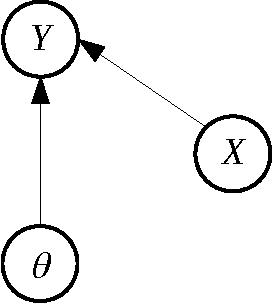
\includegraphics[width=.25\textwidth]{generative.pdf}\label{fig:generative}}
\hspace*{.2\textwidth}
\subfigure[Discriminative model]{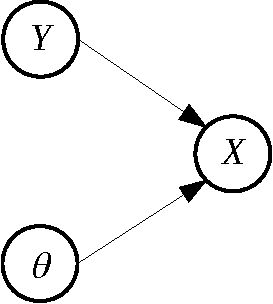
\includegraphics[width=.25\textwidth]{discriminative.pdf}\label{fig:discriminative}}
\caption{Bayesian networks representing generative and discriminative models, where $X$, $Y$ and $\theta$ respectively denote the variable of interest, the data, and the model parameters. Note the marginal independence of~$Y$ and~$\theta$ in the discriminative model.}
\label{fig:graph_comparison}
\end{center}
\end{figure}

Composite likelihood (CL, see \cite{Varin-11} and the references therein) is a semi-generative approach to statistical inference that extends the familiar notion of likelihood without requiring a full generative model. The key idea is to model an arbitrary set of low-dimensional features separately and then combine them, instead of modeling the data distribution as a whole. This may be viewed as a {\em divide and conquer} method to approximate the true but intractable likelihood. While maximum CL does not inherit the general property of maximum likelihood to yield an asymptotically minimum-variance estimator, it is consistent under mild conditions \cite{Xu-11} and may offer an excellent trade-off between computational and statistical efficiency in practice. 

In this note, CL is interpreted as a probabilistic opinion pool of ``agents'' making use of different pieces of information, or clues, extracted from the input data. Each agent acts as an isolated generative model-based statistician and expresses an opinion based on a single clue in the form of a likelihood function of the hidden variables. The agent opinions are then aggregated into a probability distribution on the hidden variables analogous to a Bayesian posterior.

We further argue that a particular log-linear opinion pool yields the best possible predictive distribution in the sense of maximum relative conditional entropy. This perspective entails a method to optimize the weights of the different agents from training data as in a typical discriminative learning scenario. 

%Something for true statisticians. Maybe we could clarify that we use the term ``Bayesian'' in the sense of ``empirical Bayesian'', implying that the parameters $\theta$ are to be estimated somehow contrary to a ``full Bayesian'' approach where they would be integrated out at inference time.


\section{Composite likelihood as opinion pooling}
\label{sec:pool}

Let $Y$ an observable multivariate random variable with sampling distribution $p(y|x)$ conditional on some unobserved variable of interest, $X\in{\cal X}$, where ${\cal X}$ is a known set. Given an experimental outcome $y$, the likelihood is the sampling distribution evaluated at $y$, seen as a function of $x$:
$$
L(x) = p(y|x)
.
$$

This requires a plausible generative model which, for complex data, may be out of reach or involve too many parameters to be estimated. A natural workaround known as {\em data reduction} is to extract some lower-dimensional representation $z=f(y)$, where $f$ is a many-to-one mapping, and consider the potentially more convenient likelihood function:
$$
\ell(x) = p(z|x)
.
$$

Substituting $L(x)$ with $\ell(x)$ boils down to restricting the sample space, thereby  ``delegating'' statistical inference to an ``agent'' provided with partial information. While it is valid for such an agent observing~$z$ only to consider $\ell(x)$ as the likelihood function of the problem, the drawback is that $\ell(x)$ might yield too vague a prediction of~$X$ due to the information loss incurred by data reduction. To make the trick statistically more efficient, we may extract several features, $z_i=f_i(y)$ for $i=1,2,\ldots,n$, and try to combine the likelihood functions $\ell_i(x) = p(z_i|x)$ that they elicit.

If we see the likelihoods as posterior distributions corresponding to uniform priors, this is a classical problem of probabilistic opinion aggregation from possibly redundant sources, for which several methods exist in the literature \cite{Tarantola-82,Genest-86,Garg-04,Allard-12}. We will show in Section~\ref{sec:maxent} that one that is particularly well-suited to our case is the {\em log-linear opinion pool}: 
\begin{equation}
\label{eq:log_pool}
p_\lambda(x|y) = \frac{1}{z_\lambda(y)} \pi(x) \prod_{i=1}^n p(z_i|x)^{\lambda_i},
\end{equation} 
where $\pi(x)$ is some reference distribution or prior, and $\lambda=(\lambda_1,\ldots,\lambda_n)$ is a vector of weights so that the normalizing factor:
$$
z_\lambda(y) = \int \pi(x) \prod_{i=1}^n p(z_i|x)^{\lambda_i} dx
$$
is finite, which holds whenever $\lambda\succeq 0$, {\em i.e.} all weights are positive, assuming that the agent opinions are always upper bounded. Negative weights should be ruled out as the existence condition $z_\lambda(y)<\infty$ would then depend on the particular opinions expressed by the agents. Also note that, while it is possible to have the weights depend on~$y$, there is a strong rational for constant weights as we shall see in the sequel. 

%Strictly positive weights guarantee the so-called 0/1 forcing property, that is, if an hypothesis~$x$ has zero likelihood according to at least one agent, then its consensus probability vanishes too.

% Not clear yet as to what a negative weight could mean!

The log-linear pool~(\ref{eq:log_pool}) bears a striking similarity to Bayes rule, yielding the form: $p_\lambda(x|y)\propto \pi(x) L^c_\lambda(x)$, where the quantity:
\begin{equation}
\label{eq:comp_lik}
L^c_\lambda(x) \equiv \prod_{i=1}^n \ell_i (x)^{\lambda_i}
\end{equation} 
plays the same role as a traditional likelihood function. This expression happens to be known in statistics as a {\em marginal composite likelihood} \cite{Varin-11}. See Appendix~\ref{sec:conditional} for the slightly more general form called {\em conditional composite likelihood}, which can be derived in the same way.

From~(\ref{eq:comp_lik}), we see that CL shares a convenient factorized form with the likelihood derived under the assumption of mutual feature independence, usually referred to as {\em na\"ive Bayes} or {\em simple Bayes} in the machine learning literature, which corresponds to the special case of unitary weights, $\lambda_1=\ldots=\lambda_n= 1$. The clear computational advantage of CL over the true likelihood is that it only requires to evaluate the marginal feature distributions rather than the joint distribution of all features.


\section{Tuning composite likelihood weights}

When the features can be considered exchangeable, it is natural to choose uniform CL weights. The CL is then a scaled version of the na\"ive Bayes likelihood, the common weight value being irrelevant to the maximum CL estimator (MCLE). The weight may be tuned so as to best adjust the pseudo posterior variance matrix to the asymptotic variance matrix of the MCLE \cite{Pauli-11}, or via a close-in-spirit curvature adjustment \cite{Ribatet-12}, in attempts to match the frequentist and composite Bayesian notions of uncertainty.

Ignoring such a goal, another frequent recommandation for CL weights is to sum up to one. This can be motivated in various ways. It turns out that the only pooling operator that does not explicitly depend on~$x$ and preserves {\em external Bayesianity} is the log-linear opinion pool with unit sum weights \cite{Genest-86b}. External Bayesianity essentially means that it should not matter whether the prior is incorporated before or after pooling, provided that all agents agree on the same prior. Another appealing property of log-linear pooling with unit sum weights is to minimize the average Kullback-Leibler (KL) divergence to the agent opinions \cite{Garg-04}. A maximum relative entropy property is also given in \cite{Wang-14}, Theorem~3.

Unit sum weights, however, correspond to the extreme situation where the features are assumed to be maximally redundant, but is clearly ineffective for independent or weakly correlated features, which require weights close to one for the CL to closely approximate the true likelihood. In this case, the CL may be much flatter than it should, leading to severly overestimated credibility sets.

{\color{red} Why is it important to fine-tune the weights?}
We therefore need a method to tune weights that can automatically adjust to the level of statistical dependence beween features.

%Instead, redundancy between agents is assumed by default, and is effectively encoded by the unit sum constraint on weights\footnote{Nevertheless, features which are {\em known} to be mutually independent can be merged into a single feature. This results in increasing their weights in the log-linear pool.}.

\section{Maxent composite likelihood}
\label{sec:maxent}

We can derive composite likelihood from the conditional maximum entropy principle \cite{BergerA-96}. It comes with a method of tuning weights, hence a particular composite likelihood function that we call maxent composite likelihood (MCL).

A cheap MaxEnt argument was already given by \cite{Wang-14}  (standard, non-conditional MaxEnt at fixed $y$, hence just an existence result but no feasible weight tuning).

What we do here is maximum {\em conditional} entropy. It's slightly more complex than a simple $I$-projection. The search space is a set of predictive distributions compatible with mean log-likelihood contraints. If I know the generative distribution, I know the expected log-likelihood.

We work with inequality constraints to force $\lambda\geq 0$:
$$
E[\log p(z_i|x)] \geq c_i \equiv \int \pi(x)p(z_i|x) \log p(z_i|x) dx dy
$$

What does the constraint mean? It means that a model is admissible if it compresses the data at least as well as all my agents. So we are not assuming that the generative models are {\em true}. We only assume that they are useful to compress the (reduced) data. Connection to MDL. 

Why not using the feature-based posteriors or Bayes factors rather than the likelihoods? It's a possibility (perhaps a connection here with Gr\"unwald's luckiness). A justification for not doing it is that the coordinator should discard the priors used by the agents. The constraints are not purely evidence-based since the moments depend on the coordinator's prior but it is arguable a mess of priors wouldn't be good.

Intuition behind weights: Lagrange multipliers to enforce a constraint... Notion of feature relevance. But does $\lambda_1>\lambda_2$ imply that $z_1$ is more relevant than $z_2$? 

The derivation assumed the marginal distribution of the data $h(y)$ to be known. In practice, it is estimated by the empirical distribution just like the moments are estimated.

Game theoretic interpretation \cite{Grunwald-04}.

The dual function boils down to the famous cross-entropy.

Single feature case ($y=z$): the maxent solution has the form $p(x|y)\propto\pi(x)p(y|x)^\lambda$. We expect to have $\lambda=1$ but it's not necessarily the case. It is if $h(y)=\int\pi(x)p(y|x)dx$ because then $h(y)p(x|y)=\pi(x)p(y|x)$ so the constraint is verified (and active). This also tells us that the data marginal should be consistent with the prior on labels for this much expected consistency property to hold. So, either weight datapoints so as to match a desired prior (e.g., uniform) or take the empirical distribution of labels as the ``prior''. 

Which brings another question: in this case, the (unique) weight is insensitive to the prior -- is it true in general? The answer is no. The weights generally depend on the prior. Hence the maxent composite likelihood is prior-dependent. This is an important conceptual difference with the classical notion of likelihood.

\section{Super composite likelihood}
\label{sec:super}

When chosen for computational simplicity, clues may not only convey limited information at individual level: their informativeness may also be very much hypothesis-dependent. Consider, for instance, diagnosing a disease from a routine medical checkup. Body temperature may point to a bacterial infection by comparison with normality, but would not help detecting a non-infectious cardiovascular disease -- and conversely for, say, blood pressure.

This motivates a more general setting where clues can be weighted differently depending on hypotheses.

What happens if we use mean-values constraints conditional on $x$ instead of jointly averaged over $x$ and $y$? This boils down to picking functions of the form:
$$
\chi(x-a)\ell_i(x,y)
$$

The answer is that the maxent solution has the form:
$$
p_\lambda(x|y) = \pi(x) \prod_i p(z_i|x)^{\lambda_i(x)}
$$

In other words, the weights become dependent on the variable of interest. This is the super composite likelihood idea.


\section{Composite EM algorithm for unsupervised learning}
\label{sec:gem}

In a nutshell: alternate unsupervised learning of partial model parameters ($M$-step) and re-estimation of label posteriors via maxent ($E$-step). 

$M$-step: given a posterior estimate $q(x|y)$, do just as if the features were independent and solve: 
$$
\max_\theta
\int \sum_i h(y)q(x|y) \log p_\theta(z_i,x) dx dy
$$

Note we can estimate cross-feature parameters such as class proportions.

Surrogate $E$-step: given generative parameters, recompute the moment constraints and update $q(x|y)$ according to the conditional maxent principle:
$$
\min_q
\int h(y)q(x|y) \log \frac{q(x|y)}{\pi(x)} dx dy
$$
s.t.
$$
\int h(y)q(x|y)\log p_\theta(z_i|x) dx dy \geq \int \pi(x)p_\theta(z_i|x)\log p_\theta(z_i|x) dx dy
$$

However, there is an important issue: how is $h(y)$ defined in both the $M$- and $E$-steps? In supervised context, $h(x,y)$ can be defined beforehand as the prior-corrected empirical distribution:
$$
h(x,y) = \pi(x) \frac{h_0(x,y)}{h_0(x)},
$$
where $h_0(x,y)$ is the raw empirical distribution. In unsupervised context, the best we can do is to replace $h_0(x,y)$ with $h_0(y)q(x|y)$, implying that the empirical distribution of $y$ is reweighted according to:
$$
h(y) = \sum_i w_i\delta(y-y_i),
\qquad
w_i = \int \pi(x)\frac{q(x|y_i)}{\sum_j q(x|y_j)} dx,
$$
which needs to be done each time $q(x|y)$ is updated, that is, after each $E$-step.

The other option is to keep $h(y)$ constant throughout the iterations but adapt $\pi(x)$ as the marginal distribution of labels learned in the $M$-step. In this case, it's no longer a ``prior''. 

Are we minimizing a unique functional as in the variational EM algorithm? Possibly not. We may see this generalization as a two-player game. One player tries to predict several data features independently. The other player tries to predict labels. Together, they find patterns (clusters) in unlabeled data. Does the more general version converge? Does the game have a value? And so on.

In the case of a single feature, is this the well-known EM? The $M$-step is clearly the same, what about the $E$-step? It is the same if $h(y)p_\theta(x|y)=p_\theta(y|x)\pi(x)$. However, this condition won't hold if $h(y)$ is an empirical distribution... In this special case, the ``E player'' could use the data distribution model produced by the ``M player'' instead of the empirical one but, more generally, there is no data distribution model so he has to stick to the empirical one.

The maxent is a surrogate for the $E$-step. It reflects the lack of a full model $p_\theta(x,y)$.

% Accounting here for Xi'An comment on xianblog.wordpress.com
% The sum of the powers is constrained to be equal to one, even though
% I do not understand why the dimensions of the projections play nog
% role in this constraint. Simplicity is advanced as an argument,
% which sounds rather weak…
%This simple constraint is implied by the external Bayesianity requirement: as it turns out, the only aggregation operator which is both externally Bayesian and independent from $x$ boils down to plugging a composite likelihood with unit sum weights into Bayes rule, hence extending the classical notion of likelihood in Bayesian analysis.


\section{Discussion}
\label{sec:discussion}

Deep learning is discriminative...

CL is a concept from computational statistics that has mainly been developed so far in a frequentist perspective as a surrogate for the maximum likelihood method. We have shown a deep connection between CL and probabilistic inference, thereby establishing CL as a class of discriminative models. Because CL is built from a set of marginal feature-specific generative distributions, it is in essence a two-step semi-generative, semi-discriminative learning approach. In the first, ``generative'' phase, the feature distributions are learned; in the second, ``discriminative'' phase, the feature weights are learned. This strategy can be thought of as a form of non-adaptive boosting.

%The first phase corresponds to the training of ``weak learners''. The second phase amounts to a form of boosting. 

A purely discriminative learning could be used instead but...
Why potentially more efficient than pure discriminative training: because generative training is always more efficient than discriminative training if models are comparable. So the key point is that ``we have less parameters in the discriminant phase". Good in small datasets. But also in asymptotic regime if the features are weakly or highly correlated (???).

Logistic regression / naive Bayes example. Under homoscedasticity (assuming that each feature has class-independent variance), CBI is equivalent to logistic regression -- because the predictive distribution family is the same. This is a case where BCI brings nothing. But consider heteroscedasticity, then BCI yields a quadratic classifier. Compared to a fully discriminative model, the number of parameters to learned in the discriminative phase is reduced by half.

The first training phase is easier if supervised but could be unsupervised too (using mixture models). How do we then deal with label switching issues? Can we safely assume conditional feature independence {\em in the generative training phase}? I believe so provided that the marginal distribution parameters are disjoint. It's obvious in the supervised learning scenario.

If unsupervised, the first learning phase could be compared with contrastive pre-training of RBMs \cite{Hinton-06,Fischer-14}, which also optimize parameters for generation of observable features. BCI is comparable with an RBM with a single output unit (which is just a generative model assuming conditionial feature independence). The key difference is that the RBM is a full generative model while BCI only deals with marginal models, hence relying on weaker assumptions. This won't change anything in the pre-training phase but RBMs have to deal with more parameters in the generative learning phase. In fully supervised context, RBM pre-training is pointless since all parameters learned in the first phase will be overwritten. In BCI, pre-training is crucial even in supervised context because the parameters learned in the discriminative phase (the feature weighs) describe a sub-manifold of the predictive distribution family.

Needs features. Not a representation learning method, but could be coupled why not.


%{\color{red} Moreover, while RBM parameters are typically refined in a supervised discriminative learning step, disjoint set of parameters for SCL. Dunno how to say that.} 

%In such context, SCL competes with classical discriminative models (logistic regression, Gaussian processes \cite{Rasmussen-06}, maximum entropy models \cite{BergerA-96}, etc.), and may compare more or less favorably in practice depending on the amount of training data. For relatively small training datasets, we may hope for more accurate inference using~SCL than using traditional discriminative models, extrapolating from the results of \cite{Ng-01} regarding the comparison between logistic regression and na\"ive Bayes classifiers.
%{\color{red}Ici, il manque la comparaison avec les RBMs qui ne sont pas (forcement) des modeles discriminatifs.}

%%, hence alleviating the need for heavily supervised model training

%In summary, CL has the potential to yield weakly supervised or unsupervised Bayesian-like inference procedures depending on the particular task at hand. This property reflects the encoding of statistical relationships between the data and {\em all} unknown parameters. CL thus appears as a trade-off between generative models, which are optimal for unsupervised learning but possibly intractable, and traditional discriminative models (logistic regression, Gaussian processes \cite{Rasmussen-06}, maximum entropy models \cite{BergerA-96}, etc.), which are inherently supervised. CL models are discriminative models assembled from atomic generative models and, from this point of view, may be considered as {\em semi-generative} models.

%CL may be considered as a {\em semi-generative} model: a discriminative model assembled from partial generative models.

%As a note of caution, we shall stress that the pre-determined weights assigned to the different associations between observed and unobserved values represent prior knowledge regarding the informativeness of clues. A poor choice of weights will inevitably result in a poor approximation to the ``true'' Bayesian posterior -- the posterior that would be obtained from a realistic generative model if it was tractable. In future work, we will investigate feature selection strategies to mitigate this problem.

% Improve the discussion on following aspects:
% ** Why is it compatible with unsupervised learning? Give more insight.
% ** Stress the contribution: class-specific weighting.
% * Pivotality argument.
% * Bayes is a special case of composite Bayes.

{\color{red}Product of fucking experts \cite{Hinton-02}. Log-linear pool to build a generative model (assuming in fact independence between experts). Better seen as a ``log-mixture model''. Sounds like each expert is associated with a class, so it's the same as a RBM. Contrastive learning approximates ML parameter estimation. The experts are learning jointly. It's just a generative model.}

{\color{red}Two-step training: generative phase then discriminative phase. Why is it cool?}

{\color{red}CBI is just a way to reweight Naive Bayes. What's the big deal? Can we really expect massively superior performance? Are we just talking about realistic credibility sets?}


\appendix

\section{Conditional composite likelihood}
\label{sec:conditional}

As a straightforward  extension of marginal CL, each feature-based likelihood may be conditioned by an additional ``independent'' feature $z^c_i = f^c_i(y)$ considered as a predictor of the ``dependent'' feature, $z_i=f_i(y)$, yielding the more general form:
\begin{equation}
\label{eq:cond_feat_lik}
\ell_i(x) = p(z_i|x,z^c_i).
\end{equation}

Conditioning may be useful if it is believed that $z^c_i$ alone is little or not informative about $x$, but can provide relevant information when considered jointly with $x$, as in the case of regression covariates, for instance. Equation~(\ref{eq:comp_lik}) then amounts to conditional CL \cite{Varin-11}, a more general form of CL also including Besag's historical {\em pseudo-likelihood} \cite{Besag-74} developed for image segmentation.


\section{Minimally discriminative model}

Let $\pi(x)$ some reference distribution that represents full
uncertainty about $X$. We wish to select the joint distribution
$p(x,y)$ that minimizes:
$$
I(p) = \int p(x,y) \log \frac{p(x|y)}{\pi(x)} dy,
$$ subject to feature mean-value constraints of the form:
$$
\int p(x,y) f(x,y) dx dy = \mu.
$$

There are two special cases of this problem in the literature.  On the
one hand, the {\em maximum entropy classifier} \cite{BergerA-96}
incorporates the constraint that $p(y)$ be known, however we will see
that this is not necessary. The {\em minimally informative likelihood}
method \cite{Yuan-99b,Yuan-99}, on the other hand, imposes that
$p(x)=\pi(x)$, hence assuming the form $p(x,y)=\pi(x)p(y|x)$. We won't
make such assumptions here and will consider the case where $\mu$ is
completely unknown.

The above problem is seen to be equivalent to minimizing the auxiliary
objective function:
$$
I(p,m) 
= \int p(x,y) \log \frac{p(x,y)}{\pi(x)m(y)} dxdy,
$$ over $p$ and $m$, subject to the same constraints on $p$. We note
that $I(p,m)=I(p)+D(p_y\|m)$, showing that the auxiliary function
essentially adds a penalty term to the actual objective in order to
force $p(y)$ close to $m(y)$.

Minimizing $I(p,m)$ along both $p$ and $m$ is basically a minimum KL
divergence problem between two convex distribution spaces, so there
must be a unique solution {\bf -- to be checked in
  \cite{Cover-91}}. It is similar to the rate-distortion problem in
information theory, which may be solved by alternate minimization,
yielding a Blahut-Arimoto algorithm.
\begin{itemize}
\item {\em Let's call it A-step}. Optimize $p(x,y)$ at fixed $m$
  s.t. constraint:
$$
\exists \lambda, \qquad
p_{\lambda,m}(x,y) = \frac{1}{Z(\lambda, m)} \pi(x) m(y) e^{-\lambda^\top t(x,y)}
$$
The actual $\lambda$ is found my maximizing the dual function
$\psi(\lambda,m)$, see below.
\item {\em Let's call it B-step}. Optimize $m(y)$ at fixed $p(x,y)$:
$$
m(y) = \int p(x,y) dx
$$
\end{itemize}

Upon convergence, the algorithm outputs both joint and marginal
distributions $p_{\star}(x,y)$ and $m_{\star}(y)$ that both depend on
$\mu$. By construction, we have that $p_{\star}(y) = m_{\star}(y)$,
therefore $p_\star(x|y)=p_{\star}(x,y)/m_{\star}(y)$.


\section{Comparison with maximum entropy classifier}

Lagrangian...
$$
{\cal L}(p,m,\lambda)
= 
\int p(x,y) \log \frac{p(x,y)}{\pi(x)m(y)} dxdy
+
\lambda^\top \left( 
\int p(x,y) f(x,y) dydy - \mu 
\right)
$$ where $\lambda$ represents a vector-valued Lagrange multiplier. At
fixed $m$, the solution has the form:
$$
p_{\lambda,m}(x,y) = \frac{1}{Z(\lambda,m)}
\pi(x) m(y) e^{-\lambda^\top f(x,y)} 
$$

Note that this implies that the conditional distribution is
independent of $m$ once $\lambda$ is determined,
$$
p_\lambda(x|y) = \frac{1}{z(\lambda,y)} \pi(x) e^{-\lambda^\top f(x,y)} 
$$

Also, the marginal is a modulation of $m(y)$:
$$
p_{\lambda,m}(y) = \frac{z(\lambda,y)}{Z(\lambda,m)} m(y)
$$

Dual function at fixed $m$:
$$
\psi(\lambda,m) 
\equiv \min_p {\cal L}(p,m,\lambda)
= 
- \log Z(\lambda,m) - \lambda^\top \mu
.
$$ 

An alternative expression is:
$$
\psi(\lambda, m)
= 
\int h(x,y) 
\log \frac{p_{\lambda,m}(x,y)}{\pi(x)m(y)} dxdy,
$$ where $h(x,y)$ is any distribution statisfying the
constraints. This shows that maximizing the dual function at fixed $m$
is essentially the same as minimizing the KL divergence
$D(h\|p_{\lambda,m})$ over $\lambda$, in other words fitting $h(x,y)$
by some distribution of the form $p_{\lambda,m}$. The fact that the
result does not depend on the particular $h(x,y)$ that is chosen, as
long as it satifies the constraint, is a general property of
exponential families.

We also have that the dual function associated with $I(p)$ reads:
\begin{eqnarray*}
\psi(\lambda) 
 & = & \min_m \psi(\lambda, m)\\
 & = & \int h(x,y) \log \frac{p_{\lambda}(x|y)}{\pi(x)} dxdy\\
 & = & -\int h(y) \log z(\lambda,y) dy - \lambda^\top \mu
\end{eqnarray*}

But, wait, that's exactly what we get in the maximum entropy
classifier! So, at the end of the day, we simply got an alternative
method to learn $\lambda$ in the maximum entropy classifier, i.e. the
Blahut-Arimoto algorithm as opposed to a brute-force maximization of
$\psi(\lambda)$. Both methods will converge to the same $\lambda$...

What it essentially means is that the optimal $\lambda$ is insensitive
to $m(y)$ as long as $m(y)$ is compliant in the sense that:
$$
m(y) = \int h(x,y) dx,
$$ for some distribution $h(x,y)$ statisfying the constraint. This is
true for the optimal $m_\star(y)$ output by the BA algorithm, but
also, for instance, for the empirical distribution of observations in
a training dataset used to estimate $\mu$, as proposed in
\cite{BergerA-96}. The only special property of $m_\star(y)$ is to
yield the full Bayesian model $p_\star(x,y)=p_\star(x|y)m_\star(y)$
that minimizes the discrimination information. We may not care too
much about that in practice since we will only use $p_\star(x|y)$. 

\section{Comparison with minimally informative likelihood}

Yuan \cite{Yuan-99} considered the situation where we add the
constraint that $p(x)=\pi(x)$ to the minimum discrimination inference
problem. Unknown is then the conditional distribution
$p(y|x)$. Lagrangian...
\begin{eqnarray*}
{\cal L}(p,m,\lambda)
 & = & 
\int \pi(x)p(y|x) \log \frac{p(y|x)}{m(y)} dxdy
+
\lambda^\top \left( 
\int \pi(x)p(y|x) f(x,y) dydy - \mu 
\right) \\
 & = & 
\int \pi(x)
\left( 
\int
p(y|x) \log \frac{p(y|x)}{m(y)} dy
+
\lambda^\top 
\int p(y|x) f(x,y) dy
- \mu 
\right)
dx 
\end{eqnarray*}

The derivative is given by,
$$
\frac{\partial\cal L}{\partial p(y|x)}
= 
\pi(x)\left[ 
1 + \log \frac{p(y|x)}{m(y)} 
+ \lambda^\top f(x,y)
\right],
$$
hence the optimal model at fixed $m$ has the form:
$$
p_{\lambda,m}(y|x) = \frac{1}{Z(\lambda,m,x)} m(y) e^{-\lambda^\top f(x,y)} 
$$

Note that the induced posterior distribution $p_{\lambda,m}(x|y)$ has
a different form from above unless the normalizing factor
$Z(\lambda,m,x)$ turns out independent from $x$. If this is not the
case, we no longer have the property that $p_{\lambda,m}(x|y)$ is
independent from $m$ given $\lambda$.

Dual function...
$$
\psi(\lambda,m) 
=
- \int \pi(x) \log Z(\lambda, m, x) dx
- \lambda^\top \mu
$$

Equivalently, for any distribution under the form $\pi(x)h(y|x)$ that
satisfies the moment constraint, we have:
$$
\psi(\lambda,m) 
=
\int \pi(x) h(y|x) \log \frac{p_{\lambda,m}(y|x)}{m(y)} dxdy
$$

Now, the real question is why should we constrain $p(x)$, which boils
down to a Bayesian prior in this context, to be the same as our
reference $\pi(x)$? It only makes sense if we want our inference to
stick to a generative modeling paradigm... but haven't we already
given up on that? Therefore, unless we find a good reason not to, we
won't impose the $p(x)=\pi(x)$ constraint, thereby allowing for a
discrepancy between the reference and the prior.


\section{Discriminative vs. semi-discriminative}

Let's go back to the equivalence we found between our approach and the
maximum entropy classifier (MCE) \cite{BergerA-96}. We have said that
the former is essentially a re-formulation of MCE.

But the re-formulation also conveys a generalization of MCE if,
instead of letting $m$ being an arbitrary distribution, we restrict
its search space to some set of acceptable reference
distributions. Would such a strategy be useful? 

Recall that the method selects the joint distribution that minimizes
discriminative information, as defined by $I(p)$:
$$
I(p) 
= \int p(x,y)\log\frac{p(x|y)}{\pi(x)} dxdy
= E_Y[D(p_{x|y}\|\pi)]
$$

The latter characterization reminds us that discriminative information
is defined in an average sense. The corresponding posterior $p(x|y)$
may not be conservative for some $y$, in particular those that are
unlikely under $p(y)$. It would be a problem if that's the case for
the particular data at hand. For that to happen rarely, the ideal
$p(y)$ would be the ``true'' marginal distribution of $Y$.

However, for vague mean value constraints, nothing may prevent the
optimal $m_\star(y)$ from departing significantly from that ideal
distribution. In fact, we can show that $m_\star(y)$ only has mass at
$y$ values that maximize $z(\lambda_\star,y)$, and is therefore likely
sparse. This is because $m_\star$ minimizes $\psi(\lambda_\star,m)$,
which is equivalent to maximizing $Z(\lambda_\star,m)$ and we have:
$$
Z(\lambda, m) = \int m(y) z(\lambda, y) dy.
$$

In other words, the solution to our problem may be singular! It does
not hurt since, as discussed above, one may alternatively fix $m(y)$
to some pre-defined distribution... but this, in practice, restricts
the method to supervised learning situations.

We may not face this issue with the MIL method, which further imposes
the prior on $X$, so all the information from the constraints goes
into specifying a possibly reasonable generative model.



\bibliographystyle{abbrv}
\bibliography{cvis,stat,alexis}

%%\documentclass[english]{scrartcl}

\usepackage{fullpage}
\usepackage{amstext,amssymb,amsmath,amsthm}
\usepackage{graphicx,subfigure}
\usepackage{multirow}
\usepackage{url}
\usepackage{hyperref}
\usepackage{color}

\graphicspath{{.}{pics/}}

%\newtheorem{theorem}{Theorem}[section]
%\newtheorem{proposition}[theorem]{Proposition}


\title{Composite Bayesian inference}
\date{}
\author{Alexis Roche\thanks{\url{alexis.roche@centraliens.net}}}

%\newcommand{\fix}{\marginpar{FIX}}
%\newcommand{\new}{\marginpar{NEW}}
%\newcommand{\matphi}{\boldsymbol{\Phi}} 
%\def\x{{\mathbf{x}}}
%\def\z{{\mathbf{z}}}
%\def\u{{\mathbf{u}}}
%\def\p{{\bar{\mathbf{p}}}}
%\def\q{{\bar{\mathbf{q}}}}



\begin{document}

\maketitle

\begin{abstract}
This note revisits the concept of composite likelihood from the perspective of probabilistic inference, and advocates a machine learning approach to tune the associated ``weights'', which stems naturally from a connection with the maximum entropy principle: the predictive distribution that maximizes conditional entropy relative to a given prior and subject to multiple mean log-likelihood inequality constraints is, up to a normalizing factor, the prior multiplied by a particular composite likelihood function, hence providing a ``composite'' extension of Bayes rule. We argue that composite Bayesian inference is a middle way between generative and discriminative approaches to statistical inference, which can be powerful in shallow learning and transfer learning problems.
\end{abstract}


\section{Introduction}
\label{sec:intro}

Classical frequentist and Bayesian inference paradigms rest upon the existence of a probabilistic data-generating model that is both empirically valid and computationally tractable. Because this is challenging for complex data, other inference models are commonly used in applied science: deliberately misspecified generative models, as in quasi-likelihood methods \cite{White-82,Walker-13} or na\"ive Bayes \cite{Ng-01}; data compression models as in minimum description length \cite{Grunwald-07}; and discriminative models\footnote{A {\em discriminative} model is a parametric family that describes the distribution of a variable of interest conditional on data, in contrast with a {\em generative} model, which describes the conditional distribution of data given the variable of interest.}, which currently dominate the field of artificial intelligence and typically require massive supervised learning -- these include classical techniques (maximum entropy classifiers \cite{BergerA-96}, support vector machines \cite{Vapnik-00}, Gaussian processes \cite{Rasmussen-06}) as well as most deep learning techniques \cite{Lecun-15,Goodfellow-16} with the exception of deep belief networks \cite{Hinton-06,Fischer-14}. 

A strong limitation of discriminative models is that they are not suitable for unsupervised learning or on-the-fly parameter estimation because they treat the data and the model parameters as {\em marginally independent}, meaning that the data conveys no information about the parameters unless the variable of interest is observed. This is illustrated in Figure~\ref{fig:graph_comparison} by the respective directed graph representations of generative and discriminative models. For the same reason, supervised learning in a discriminative model is less precise than in a generative model spanning the same family of posteriors, hence it is less effective in small training sets \cite{Ng-01}. Overall, pure discriminative models are of little use outside the context of big labeled data.

% p(x,y|theta) = p(x|y,theta)p(y|theta)

\begin{figure}[!ht]
\begin{center}
\subfigure[Generative model]{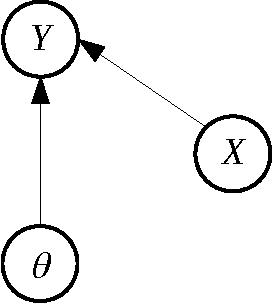
\includegraphics[width=.25\textwidth]{generative.pdf}\label{fig:generative}}
\hspace*{.2\textwidth}
\subfigure[Discriminative model]{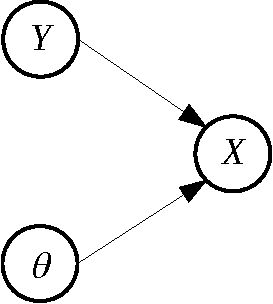
\includegraphics[width=.25\textwidth]{discriminative.pdf}\label{fig:discriminative}}
\caption{Bayesian networks representing generative and discriminative models, where $X$, $Y$ and $\theta$ respectively denote the variable of interest, the data, and the model parameters. Note the marginal independence of~$Y$ and~$\theta$ in the discriminative model.}
\label{fig:graph_comparison}
\end{center}
\end{figure}

Composite likelihood (CL, see \cite{Varin-11} and the references therein) is a semi-generative approach to statistical inference that extends the familiar notion of likelihood without requiring a full generative model. The key idea is to model an arbitrary set of low-dimensional features separately and then combine them, instead of modeling the data distribution as a whole. This may be viewed as a {\em divide and conquer} method to approximate the true but intractable likelihood. While maximum CL does not inherit the general property of maximum likelihood to yield an asymptotically minimum-variance estimator, it is consistent under mild conditions \cite{Xu-11} and may offer an excellent trade-off between computational and statistical efficiency in practice. 

In this note, CL is interpreted as a probabilistic opinion pool of ``agents'' making use of different pieces of information, or clues, extracted from the input data. Each agent acts as an isolated generative model-based statistician and expresses an opinion based on a single clue in the form of a likelihood function of the hidden variables. The agent opinions are then aggregated into a probability distribution on the hidden variables analogous to a Bayesian posterior.

We further argue that a particular log-linear opinion pool yields the best possible predictive distribution in the sense of maximum relative conditional entropy. This perspective entails a method to optimize the weights of the different agents from training data as in a typical discriminative learning scenario. 

%Something for true statisticians. Maybe we could clarify that we use the term ``Bayesian'' in the sense of ``empirical Bayesian'', implying that the parameters $\theta$ are to be estimated somehow contrary to a ``full Bayesian'' approach where they would be integrated out at inference time.


\section{Composite likelihood as opinion pooling}
\label{sec:pool}

Let $Y$ an observable multivariate random variable with sampling distribution $p(y|x)$ conditional on some unobserved variable of interest, $X\in{\cal X}$, where ${\cal X}$ is a known set. Given an experimental outcome $y$, the likelihood is the sampling distribution evaluated at $y$, seen as a function of $x$:
$$
L(x) = p(y|x)
.
$$

This requires a plausible generative model which, for complex data, may be out of reach or involve too many parameters to be estimated. A natural workaround known as {\em data reduction} is to extract some lower-dimensional representation $z=f(y)$, where $f$ is a many-to-one mapping, and consider the potentially more convenient likelihood function:
$$
\ell(x) = p(z|x)
.
$$

Substituting $L(x)$ with $\ell(x)$ boils down to restricting the sample space, thereby  ``delegating'' statistical inference to an ``agent'' provided with partial information. While it is valid for such an agent observing~$z$ only to consider $\ell(x)$ as the likelihood function of the problem, the drawback is that $\ell(x)$ might yield too vague a prediction of~$X$ due to the information loss incurred by data reduction. To make the trick statistically more efficient, we may extract several features, $z_i=f_i(y)$ for $i=1,2,\ldots,n$, and try to combine the likelihood functions $\ell_i(x) = p(z_i|x)$ that they elicit.

If we see the likelihoods as posterior distributions corresponding to uniform priors, this is a classical problem of probabilistic opinion aggregation from possibly redundant sources, for which several methods exist in the literature \cite{Tarantola-82,Genest-86,Garg-04,Allard-12}. We will show in Section~\ref{sec:maxent} that one that is particularly well-suited to our case is the {\em log-linear opinion pool}: 
\begin{equation}
\label{eq:log_pool}
p_\lambda(x|y) = \frac{1}{z_\lambda(y)} \pi(x) \prod_{i=1}^n p(z_i|x)^{\lambda_i},
\end{equation} 
where $\pi(x)$ is some reference distribution or prior, and $\lambda=(\lambda_1,\ldots,\lambda_n)$ is a vector of weights so that the normalizing factor:
$$
z_\lambda(y) = \int \pi(x) \prod_{i=1}^n p(z_i|x)^{\lambda_i} dx
$$
is finite, which holds whenever $\lambda\succeq 0$, {\em i.e.} all weights are positive, assuming that the agent opinions are always upper bounded. Negative weights should be ruled out as the existence condition $z_\lambda(y)<\infty$ would then depend on the particular opinions expressed by the agents. Also note that, while it is possible to have the weights depend on~$y$, there is a strong rational for constant weights as we shall see in the sequel. 

%Strictly positive weights guarantee the so-called 0/1 forcing property, that is, if an hypothesis~$x$ has zero likelihood according to at least one agent, then its consensus probability vanishes too.

% Not clear yet as to what a negative weight could mean!

The log-linear pool~(\ref{eq:log_pool}) bears a striking similarity to Bayes rule, yielding the form: $p_\lambda(x|y)\propto \pi(x) L^c_\lambda(x)$, where the quantity:
\begin{equation}
\label{eq:comp_lik}
L^c_\lambda(x) \equiv \prod_{i=1}^n \ell_i (x)^{\lambda_i}
\end{equation} 
plays the same role as a traditional likelihood function. This expression happens to be known in statistics as a {\em marginal composite likelihood} \cite{Varin-11}. See Appendix~\ref{sec:conditional} for the slightly more general form called {\em conditional composite likelihood}, which can be derived in the same way.

From~(\ref{eq:comp_lik}), we see that CL shares a convenient factorized form with the likelihood derived under the assumption of mutual feature independence, usually referred to as {\em na\"ive Bayes} or {\em simple Bayes} in the machine learning literature, which corresponds to the special case of unitary weights, $\lambda_1=\ldots=\lambda_n= 1$. The clear computational advantage of CL over the true likelihood is that it only requires to evaluate the marginal feature distributions rather than the joint distribution of all features.


\section{Tuning composite likelihood weights}

When the features can be considered exchangeable, it is natural to choose uniform CL weights. The CL is then a scaled version of the na\"ive Bayes likelihood, the common weight value being irrelevant to the maximum CL estimator (MCLE). The weight may be tuned so as to best adjust the pseudo posterior variance matrix to the asymptotic variance matrix of the MCLE \cite{Pauli-11}, or via a close-in-spirit curvature adjustment \cite{Ribatet-12}, in attempts to match the frequentist and composite Bayesian notions of uncertainty.

Ignoring such a goal, another frequent recommandation for CL weights is to sum up to one. This can be motivated in various ways. It turns out that the only pooling operator that does not explicitly depend on~$x$ and preserves {\em external Bayesianity} is the log-linear opinion pool with unit sum weights \cite{Genest-86b}. External Bayesianity essentially means that it should not matter whether the prior is incorporated before or after pooling, provided that all agents agree on the same prior. Another appealing property of log-linear pooling with unit sum weights is to minimize the average Kullback-Leibler (KL) divergence to the agent opinions \cite{Garg-04}. A maximum relative entropy property is also given in \cite{Wang-14}, Theorem~3.

Unit sum weights, however, correspond to the extreme situation where the features are assumed to be maximally redundant, but is clearly ineffective for independent or weakly correlated features, which require weights close to one for the CL to closely approximate the true likelihood. In this case, the CL may be much flatter than it should, leading to severly overestimated credibility sets.

{\color{red} Why is it important to fine-tune the weights?}
We therefore need a method to tune weights that can automatically adjust to the level of statistical dependence beween features.

%Instead, redundancy between agents is assumed by default, and is effectively encoded by the unit sum constraint on weights\footnote{Nevertheless, features which are {\em known} to be mutually independent can be merged into a single feature. This results in increasing their weights in the log-linear pool.}.

\section{Maxent composite likelihood}
\label{sec:maxent}

We can derive composite likelihood from the conditional maximum entropy principle \cite{BergerA-96}. It comes with a method of tuning weights, hence a particular composite likelihood function that we call maxent composite likelihood (MCL).

A cheap MaxEnt argument was already given by \cite{Wang-14}  (standard, non-conditional MaxEnt at fixed $y$, hence just an existence result but no feasible weight tuning).

What we do here is maximum {\em conditional} entropy. It's slightly more complex than a simple $I$-projection. The search space is a set of predictive distributions compatible with mean log-likelihood contraints. If I know the generative distribution, I know the expected log-likelihood.

We work with inequality constraints to force $\lambda\geq 0$:
$$
E[\log p(z_i|x)] \geq c_i \equiv \int \pi(x)p(z_i|x) \log p(z_i|x) dx dy
$$

What does the constraint mean? It means that a model is admissible if it compresses the data at least as well as all my agents. So we are not assuming that the generative models are {\em true}. We only assume that they are useful to compress the (reduced) data. Connection to MDL. 

Why not using the feature-based posteriors or Bayes factors rather than the likelihoods? It's a possibility (perhaps a connection here with Gr\"unwald's luckiness). A justification for not doing it is that the coordinator should discard the priors used by the agents. The constraints are not purely evidence-based since the moments depend on the coordinator's prior but it is arguable a mess of priors wouldn't be good.

Intuition behind weights: Lagrange multipliers to enforce a constraint... Notion of feature relevance. But does $\lambda_1>\lambda_2$ imply that $z_1$ is more relevant than $z_2$? 

The derivation assumed the marginal distribution of the data $h(y)$ to be known. In practice, it is estimated by the empirical distribution just like the moments are estimated.

Game theoretic interpretation \cite{Grunwald-04}.

The dual function boils down to the famous cross-entropy.

Single feature case ($y=z$): the maxent solution has the form $p(x|y)\propto\pi(x)p(y|x)^\lambda$. We expect to have $\lambda=1$ but it's not necessarily the case. It is if $h(y)=\int\pi(x)p(y|x)dx$ because then $h(y)p(x|y)=\pi(x)p(y|x)$ so the constraint is verified (and active). This also tells us that the data marginal should be consistent with the prior on labels for this much expected consistency property to hold. So, either weight datapoints so as to match a desired prior (e.g., uniform) or take the empirical distribution of labels as the ``prior''. 

Which brings another question: in this case, the (unique) weight is insensitive to the prior -- is it true in general? The answer is no. The weights generally depend on the prior. Hence the maxent composite likelihood is prior-dependent. This is an important conceptual difference with the classical notion of likelihood.

\section{Super composite likelihood}
\label{sec:super}

When chosen for computational simplicity, clues may not only convey limited information at individual level: their informativeness may also be very much hypothesis-dependent. Consider, for instance, diagnosing a disease from a routine medical checkup. Body temperature may point to a bacterial infection by comparison with normality, but would not help detecting a non-infectious cardiovascular disease -- and conversely for, say, blood pressure.

This motivates a more general setting where clues can be weighted differently depending on hypotheses.

What happens if we use mean-values constraints conditional on $x$ instead of jointly averaged over $x$ and $y$? This boils down to picking functions of the form:
$$
\chi(x-a)\ell_i(x,y)
$$

The answer is that the maxent solution has the form:
$$
p_\lambda(x|y) = \pi(x) \prod_i p(z_i|x)^{\lambda_i(x)}
$$

In other words, the weights become dependent on the variable of interest. This is the super composite likelihood idea.


\section{Composite EM algorithm for unsupervised learning}
\label{sec:gem}

In a nutshell: alternate unsupervised learning of partial model parameters ($M$-step) and re-estimation of label posteriors via maxent ($E$-step). 

$M$-step: given a posterior estimate $q(x|y)$, do just as if the features were independent and solve: 
$$
\max_\theta
\int \sum_i h(y)q(x|y) \log p_\theta(z_i,x) dx dy
$$

Note we can estimate cross-feature parameters such as class proportions.

Surrogate $E$-step: given generative parameters, recompute the moment constraints and update $q(x|y)$ according to the conditional maxent principle:
$$
\min_q
\int h(y)q(x|y) \log \frac{q(x|y)}{\pi(x)} dx dy
$$
s.t.
$$
\int h(y)q(x|y)\log p_\theta(z_i|x) dx dy \geq \int \pi(x)p_\theta(z_i|x)\log p_\theta(z_i|x) dx dy
$$

However, there is an important issue: how is $h(y)$ defined in both the $M$- and $E$-steps? In supervised context, $h(x,y)$ can be defined beforehand as the prior-corrected empirical distribution:
$$
h(x,y) = \pi(x) \frac{h_0(x,y)}{h_0(x)},
$$
where $h_0(x,y)$ is the raw empirical distribution. In unsupervised context, the best we can do is to replace $h_0(x,y)$ with $h_0(y)q(x|y)$, implying that the empirical distribution of $y$ is reweighted according to:
$$
h(y) = \sum_i w_i\delta(y-y_i),
\qquad
w_i = \int \pi(x)\frac{q(x|y_i)}{\sum_j q(x|y_j)} dx,
$$
which needs to be done each time $q(x|y)$ is updated, that is, after each $E$-step.

The other option is to keep $h(y)$ constant throughout the iterations but adapt $\pi(x)$ as the marginal distribution of labels learned in the $M$-step. In this case, it's no longer a ``prior''. 

Are we minimizing a unique functional as in the variational EM algorithm? Possibly not. We may see this generalization as a two-player game. One player tries to predict several data features independently. The other player tries to predict labels. Together, they find patterns (clusters) in unlabeled data. Does the more general version converge? Does the game have a value? And so on.

In the case of a single feature, is this the well-known EM? The $M$-step is clearly the same, what about the $E$-step? It is the same if $h(y)p_\theta(x|y)=p_\theta(y|x)\pi(x)$. However, this condition won't hold if $h(y)$ is an empirical distribution... In this special case, the ``E player'' could use the data distribution model produced by the ``M player'' instead of the empirical one but, more generally, there is no data distribution model so he has to stick to the empirical one.

The maxent is a surrogate for the $E$-step. It reflects the lack of a full model $p_\theta(x,y)$.

% Accounting here for Xi'An comment on xianblog.wordpress.com
% The sum of the powers is constrained to be equal to one, even though
% I do not understand why the dimensions of the projections play nog
% role in this constraint. Simplicity is advanced as an argument,
% which sounds rather weak…
%This simple constraint is implied by the external Bayesianity requirement: as it turns out, the only aggregation operator which is both externally Bayesian and independent from $x$ boils down to plugging a composite likelihood with unit sum weights into Bayes rule, hence extending the classical notion of likelihood in Bayesian analysis.


\section{Discussion}
\label{sec:discussion}

Deep learning is discriminative...

CL is a concept from computational statistics that has mainly been developed so far in a frequentist perspective as a surrogate for the maximum likelihood method. We have shown a deep connection between CL and probabilistic inference, thereby establishing CL as a class of discriminative models. Because CL is built from a set of marginal feature-specific generative distributions, it is in essence a two-step semi-generative, semi-discriminative learning approach. In the first, ``generative'' phase, the feature distributions are learned; in the second, ``discriminative'' phase, the feature weights are learned. This strategy can be thought of as a form of non-adaptive boosting.

%The first phase corresponds to the training of ``weak learners''. The second phase amounts to a form of boosting. 

A purely discriminative learning could be used instead but...
Why potentially more efficient than pure discriminative training: because generative training is always more efficient than discriminative training if models are comparable. So the key point is that ``we have less parameters in the discriminant phase". Good in small datasets. But also in asymptotic regime if the features are weakly or highly correlated (???).

Logistic regression / naive Bayes example. Under homoscedasticity (assuming that each feature has class-independent variance), CBI is equivalent to logistic regression -- because the predictive distribution family is the same. This is a case where BCI brings nothing. But consider heteroscedasticity, then BCI yields a quadratic classifier. Compared to a fully discriminative model, the number of parameters to learned in the discriminative phase is reduced by half.

The first training phase is easier if supervised but could be unsupervised too (using mixture models). How do we then deal with label switching issues? Can we safely assume conditional feature independence {\em in the generative training phase}? I believe so provided that the marginal distribution parameters are disjoint. It's obvious in the supervised learning scenario.

If unsupervised, the first learning phase could be compared with contrastive pre-training of RBMs \cite{Hinton-06,Fischer-14}, which also optimize parameters for generation of observable features. BCI is comparable with an RBM with a single output unit (which is just a generative model assuming conditionial feature independence). The key difference is that the RBM is a full generative model while BCI only deals with marginal models, hence relying on weaker assumptions. This won't change anything in the pre-training phase but RBMs have to deal with more parameters in the generative learning phase. In fully supervised context, RBM pre-training is pointless since all parameters learned in the first phase will be overwritten. In BCI, pre-training is crucial even in supervised context because the parameters learned in the discriminative phase (the feature weighs) describe a sub-manifold of the predictive distribution family.

Needs features. Not a representation learning method, but could be coupled why not.


%{\color{red} Moreover, while RBM parameters are typically refined in a supervised discriminative learning step, disjoint set of parameters for SCL. Dunno how to say that.} 

%In such context, SCL competes with classical discriminative models (logistic regression, Gaussian processes \cite{Rasmussen-06}, maximum entropy models \cite{BergerA-96}, etc.), and may compare more or less favorably in practice depending on the amount of training data. For relatively small training datasets, we may hope for more accurate inference using~SCL than using traditional discriminative models, extrapolating from the results of \cite{Ng-01} regarding the comparison between logistic regression and na\"ive Bayes classifiers.
%{\color{red}Ici, il manque la comparaison avec les RBMs qui ne sont pas (forcement) des modeles discriminatifs.}

%%, hence alleviating the need for heavily supervised model training

%In summary, CL has the potential to yield weakly supervised or unsupervised Bayesian-like inference procedures depending on the particular task at hand. This property reflects the encoding of statistical relationships between the data and {\em all} unknown parameters. CL thus appears as a trade-off between generative models, which are optimal for unsupervised learning but possibly intractable, and traditional discriminative models (logistic regression, Gaussian processes \cite{Rasmussen-06}, maximum entropy models \cite{BergerA-96}, etc.), which are inherently supervised. CL models are discriminative models assembled from atomic generative models and, from this point of view, may be considered as {\em semi-generative} models.

%CL may be considered as a {\em semi-generative} model: a discriminative model assembled from partial generative models.

%As a note of caution, we shall stress that the pre-determined weights assigned to the different associations between observed and unobserved values represent prior knowledge regarding the informativeness of clues. A poor choice of weights will inevitably result in a poor approximation to the ``true'' Bayesian posterior -- the posterior that would be obtained from a realistic generative model if it was tractable. In future work, we will investigate feature selection strategies to mitigate this problem.

% Improve the discussion on following aspects:
% ** Why is it compatible with unsupervised learning? Give more insight.
% ** Stress the contribution: class-specific weighting.
% * Pivotality argument.
% * Bayes is a special case of composite Bayes.

{\color{red}Product of fucking experts \cite{Hinton-02}. Log-linear pool to build a generative model (assuming in fact independence between experts). Better seen as a ``log-mixture model''. Sounds like each expert is associated with a class, so it's the same as a RBM. Contrastive learning approximates ML parameter estimation. The experts are learning jointly. It's just a generative model.}

{\color{red}Two-step training: generative phase then discriminative phase. Why is it cool?}

{\color{red}CBI is just a way to reweight Naive Bayes. What's the big deal? Can we really expect massively superior performance? Are we just talking about realistic credibility sets?}


\appendix

\section{Conditional composite likelihood}
\label{sec:conditional}

As a straightforward  extension of marginal CL, each feature-based likelihood may be conditioned by an additional ``independent'' feature $z^c_i = f^c_i(y)$ considered as a predictor of the ``dependent'' feature, $z_i=f_i(y)$, yielding the more general form:
\begin{equation}
\label{eq:cond_feat_lik}
\ell_i(x) = p(z_i|x,z^c_i).
\end{equation}

Conditioning may be useful if it is believed that $z^c_i$ alone is little or not informative about $x$, but can provide relevant information when considered jointly with $x$, as in the case of regression covariates, for instance. Equation~(\ref{eq:comp_lik}) then amounts to conditional CL \cite{Varin-11}, a more general form of CL also including Besag's historical {\em pseudo-likelihood} \cite{Besag-74} developed for image segmentation.


\section{Minimally discriminative model}

Let $\pi(x)$ some reference distribution that represents full
uncertainty about $X$. We wish to select the joint distribution
$p(x,y)$ that minimizes:
$$
I(p) = \int p(x,y) \log \frac{p(x|y)}{\pi(x)} dy,
$$ subject to feature mean-value constraints of the form:
$$
\int p(x,y) f(x,y) dx dy = \mu.
$$

There are two special cases of this problem in the literature.  On the
one hand, the {\em maximum entropy classifier} \cite{BergerA-96}
incorporates the constraint that $p(y)$ be known, however we will see
that this is not necessary. The {\em minimally informative likelihood}
method \cite{Yuan-99b,Yuan-99}, on the other hand, imposes that
$p(x)=\pi(x)$, hence assuming the form $p(x,y)=\pi(x)p(y|x)$. We won't
make such assumptions here and will consider the case where $\mu$ is
completely unknown.

The above problem is seen to be equivalent to minimizing the auxiliary
objective function:
$$
I(p,m) 
= \int p(x,y) \log \frac{p(x,y)}{\pi(x)m(y)} dxdy,
$$ over $p$ and $m$, subject to the same constraints on $p$. We note
that $I(p,m)=I(p)+D(p_y\|m)$, showing that the auxiliary function
essentially adds a penalty term to the actual objective in order to
force $p(y)$ close to $m(y)$.

Minimizing $I(p,m)$ along both $p$ and $m$ is basically a minimum KL
divergence problem between two convex distribution spaces, so there
must be a unique solution {\bf -- to be checked in
  \cite{Cover-91}}. It is similar to the rate-distortion problem in
information theory, which may be solved by alternate minimization,
yielding a Blahut-Arimoto algorithm.
\begin{itemize}
\item {\em Let's call it A-step}. Optimize $p(x,y)$ at fixed $m$
  s.t. constraint:
$$
\exists \lambda, \qquad
p_{\lambda,m}(x,y) = \frac{1}{Z(\lambda, m)} \pi(x) m(y) e^{-\lambda^\top t(x,y)}
$$
The actual $\lambda$ is found my maximizing the dual function
$\psi(\lambda,m)$, see below.
\item {\em Let's call it B-step}. Optimize $m(y)$ at fixed $p(x,y)$:
$$
m(y) = \int p(x,y) dx
$$
\end{itemize}

Upon convergence, the algorithm outputs both joint and marginal
distributions $p_{\star}(x,y)$ and $m_{\star}(y)$ that both depend on
$\mu$. By construction, we have that $p_{\star}(y) = m_{\star}(y)$,
therefore $p_\star(x|y)=p_{\star}(x,y)/m_{\star}(y)$.


\section{Comparison with maximum entropy classifier}

Lagrangian...
$$
{\cal L}(p,m,\lambda)
= 
\int p(x,y) \log \frac{p(x,y)}{\pi(x)m(y)} dxdy
+
\lambda^\top \left( 
\int p(x,y) f(x,y) dydy - \mu 
\right)
$$ where $\lambda$ represents a vector-valued Lagrange multiplier. At
fixed $m$, the solution has the form:
$$
p_{\lambda,m}(x,y) = \frac{1}{Z(\lambda,m)}
\pi(x) m(y) e^{-\lambda^\top f(x,y)} 
$$

Note that this implies that the conditional distribution is
independent of $m$ once $\lambda$ is determined,
$$
p_\lambda(x|y) = \frac{1}{z(\lambda,y)} \pi(x) e^{-\lambda^\top f(x,y)} 
$$

Also, the marginal is a modulation of $m(y)$:
$$
p_{\lambda,m}(y) = \frac{z(\lambda,y)}{Z(\lambda,m)} m(y)
$$

Dual function at fixed $m$:
$$
\psi(\lambda,m) 
\equiv \min_p {\cal L}(p,m,\lambda)
= 
- \log Z(\lambda,m) - \lambda^\top \mu
.
$$ 

An alternative expression is:
$$
\psi(\lambda, m)
= 
\int h(x,y) 
\log \frac{p_{\lambda,m}(x,y)}{\pi(x)m(y)} dxdy,
$$ where $h(x,y)$ is any distribution statisfying the
constraints. This shows that maximizing the dual function at fixed $m$
is essentially the same as minimizing the KL divergence
$D(h\|p_{\lambda,m})$ over $\lambda$, in other words fitting $h(x,y)$
by some distribution of the form $p_{\lambda,m}$. The fact that the
result does not depend on the particular $h(x,y)$ that is chosen, as
long as it satifies the constraint, is a general property of
exponential families.

We also have that the dual function associated with $I(p)$ reads:
\begin{eqnarray*}
\psi(\lambda) 
 & = & \min_m \psi(\lambda, m)\\
 & = & \int h(x,y) \log \frac{p_{\lambda}(x|y)}{\pi(x)} dxdy\\
 & = & -\int h(y) \log z(\lambda,y) dy - \lambda^\top \mu
\end{eqnarray*}

But, wait, that's exactly what we get in the maximum entropy
classifier! So, at the end of the day, we simply got an alternative
method to learn $\lambda$ in the maximum entropy classifier, i.e. the
Blahut-Arimoto algorithm as opposed to a brute-force maximization of
$\psi(\lambda)$. Both methods will converge to the same $\lambda$...

What it essentially means is that the optimal $\lambda$ is insensitive
to $m(y)$ as long as $m(y)$ is compliant in the sense that:
$$
m(y) = \int h(x,y) dx,
$$ for some distribution $h(x,y)$ statisfying the constraint. This is
true for the optimal $m_\star(y)$ output by the BA algorithm, but
also, for instance, for the empirical distribution of observations in
a training dataset used to estimate $\mu$, as proposed in
\cite{BergerA-96}. The only special property of $m_\star(y)$ is to
yield the full Bayesian model $p_\star(x,y)=p_\star(x|y)m_\star(y)$
that minimizes the discrimination information. We may not care too
much about that in practice since we will only use $p_\star(x|y)$. 

\section{Comparison with minimally informative likelihood}

Yuan \cite{Yuan-99} considered the situation where we add the
constraint that $p(x)=\pi(x)$ to the minimum discrimination inference
problem. Unknown is then the conditional distribution
$p(y|x)$. Lagrangian...
\begin{eqnarray*}
{\cal L}(p,m,\lambda)
 & = & 
\int \pi(x)p(y|x) \log \frac{p(y|x)}{m(y)} dxdy
+
\lambda^\top \left( 
\int \pi(x)p(y|x) f(x,y) dydy - \mu 
\right) \\
 & = & 
\int \pi(x)
\left( 
\int
p(y|x) \log \frac{p(y|x)}{m(y)} dy
+
\lambda^\top 
\int p(y|x) f(x,y) dy
- \mu 
\right)
dx 
\end{eqnarray*}

The derivative is given by,
$$
\frac{\partial\cal L}{\partial p(y|x)}
= 
\pi(x)\left[ 
1 + \log \frac{p(y|x)}{m(y)} 
+ \lambda^\top f(x,y)
\right],
$$
hence the optimal model at fixed $m$ has the form:
$$
p_{\lambda,m}(y|x) = \frac{1}{Z(\lambda,m,x)} m(y) e^{-\lambda^\top f(x,y)} 
$$

Note that the induced posterior distribution $p_{\lambda,m}(x|y)$ has
a different form from above unless the normalizing factor
$Z(\lambda,m,x)$ turns out independent from $x$. If this is not the
case, we no longer have the property that $p_{\lambda,m}(x|y)$ is
independent from $m$ given $\lambda$.

Dual function...
$$
\psi(\lambda,m) 
=
- \int \pi(x) \log Z(\lambda, m, x) dx
- \lambda^\top \mu
$$

Equivalently, for any distribution under the form $\pi(x)h(y|x)$ that
satisfies the moment constraint, we have:
$$
\psi(\lambda,m) 
=
\int \pi(x) h(y|x) \log \frac{p_{\lambda,m}(y|x)}{m(y)} dxdy
$$

Now, the real question is why should we constrain $p(x)$, which boils
down to a Bayesian prior in this context, to be the same as our
reference $\pi(x)$? It only makes sense if we want our inference to
stick to a generative modeling paradigm... but haven't we already
given up on that? Therefore, unless we find a good reason not to, we
won't impose the $p(x)=\pi(x)$ constraint, thereby allowing for a
discrepancy between the reference and the prior.


\section{Discriminative vs. semi-discriminative}

Let's go back to the equivalence we found between our approach and the
maximum entropy classifier (MCE) \cite{BergerA-96}. We have said that
the former is essentially a re-formulation of MCE.

But the re-formulation also conveys a generalization of MCE if,
instead of letting $m$ being an arbitrary distribution, we restrict
its search space to some set of acceptable reference
distributions. Would such a strategy be useful? 

Recall that the method selects the joint distribution that minimizes
discriminative information, as defined by $I(p)$:
$$
I(p) 
= \int p(x,y)\log\frac{p(x|y)}{\pi(x)} dxdy
= E_Y[D(p_{x|y}\|\pi)]
$$

The latter characterization reminds us that discriminative information
is defined in an average sense. The corresponding posterior $p(x|y)$
may not be conservative for some $y$, in particular those that are
unlikely under $p(y)$. It would be a problem if that's the case for
the particular data at hand. For that to happen rarely, the ideal
$p(y)$ would be the ``true'' marginal distribution of $Y$.

However, for vague mean value constraints, nothing may prevent the
optimal $m_\star(y)$ from departing significantly from that ideal
distribution. In fact, we can show that $m_\star(y)$ only has mass at
$y$ values that maximize $z(\lambda_\star,y)$, and is therefore likely
sparse. This is because $m_\star$ minimizes $\psi(\lambda_\star,m)$,
which is equivalent to maximizing $Z(\lambda_\star,m)$ and we have:
$$
Z(\lambda, m) = \int m(y) z(\lambda, y) dy.
$$

In other words, the solution to our problem may be singular! It does
not hurt since, as discussed above, one may alternatively fix $m(y)$
to some pre-defined distribution... but this, in practice, restricts
the method to supervised learning situations.

We may not face this issue with the MIL method, which further imposes
the prior on $X$, so all the information from the constraints goes
into specifying a possibly reasonable generative model.



\bibliographystyle{abbrv}
\bibliography{cvis,stat,alexis}

%%\documentclass[english]{scrartcl}

\usepackage{fullpage}
\usepackage{amstext,amssymb,amsmath,amsthm}
\usepackage{graphicx,subfigure}
\usepackage{multirow}
\usepackage{url}
\usepackage{hyperref}
\usepackage{color}

\graphicspath{{.}{pics/}}

%\newtheorem{theorem}{Theorem}[section]
%\newtheorem{proposition}[theorem]{Proposition}


\title{Composite Bayesian inference}
\date{}
\author{Alexis Roche\thanks{\url{alexis.roche@centraliens.net}}}

%\newcommand{\fix}{\marginpar{FIX}}
%\newcommand{\new}{\marginpar{NEW}}
%\newcommand{\matphi}{\boldsymbol{\Phi}} 
%\def\x{{\mathbf{x}}}
%\def\z{{\mathbf{z}}}
%\def\u{{\mathbf{u}}}
%\def\p{{\bar{\mathbf{p}}}}
%\def\q{{\bar{\mathbf{q}}}}



\begin{document}

\maketitle

\begin{abstract}
This note revisits the concept of composite likelihood from the perspective of probabilistic inference, and advocates a machine learning approach to tune the associated ``weights'', which stems naturally from a connection with the maximum entropy principle: the predictive distribution that maximizes conditional entropy relative to a given prior and subject to multiple mean log-likelihood inequality constraints is, up to a normalizing factor, the prior multiplied by a particular composite likelihood function, hence providing a ``composite'' extension of Bayes rule. We argue that composite Bayesian inference is a middle way between generative and discriminative approaches to statistical inference, which can be powerful in shallow learning and transfer learning problems.
\end{abstract}


\section{Introduction}
\label{sec:intro}

Classical frequentist and Bayesian inference paradigms rest upon the existence of a probabilistic data-generating model that is both empirically valid and computationally tractable. Because this is challenging for complex data, other inference models are commonly used in applied science: deliberately misspecified generative models, as in quasi-likelihood methods \cite{White-82,Walker-13} or na\"ive Bayes \cite{Ng-01}; data compression models as in minimum description length \cite{Grunwald-07}; and discriminative models\footnote{A {\em discriminative} model is a parametric family that describes the distribution of a variable of interest conditional on data, in contrast with a {\em generative} model, which describes the conditional distribution of data given the variable of interest.}, which currently dominate the field of artificial intelligence and typically require massive supervised learning -- these include classical techniques (maximum entropy classifiers \cite{BergerA-96}, support vector machines \cite{Vapnik-00}, Gaussian processes \cite{Rasmussen-06}) as well as most deep learning techniques \cite{Lecun-15,Goodfellow-16} with the exception of deep belief networks \cite{Hinton-06,Fischer-14}. 

A strong limitation of discriminative models is that they are not suitable for unsupervised learning or on-the-fly parameter estimation because they treat the data and the model parameters as {\em marginally independent}, meaning that the data conveys no information about the parameters unless the variable of interest is observed. This is illustrated in Figure~\ref{fig:graph_comparison} by the respective directed graph representations of generative and discriminative models. For the same reason, supervised learning in a discriminative model is less precise than in a generative model spanning the same family of posteriors, hence it is less effective in small training sets \cite{Ng-01}. Overall, pure discriminative models are of little use outside the context of big labeled data.

% p(x,y|theta) = p(x|y,theta)p(y|theta)

\begin{figure}[!ht]
\begin{center}
\subfigure[Generative model]{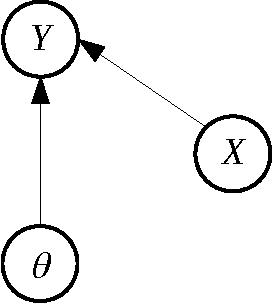
\includegraphics[width=.25\textwidth]{generative.pdf}\label{fig:generative}}
\hspace*{.2\textwidth}
\subfigure[Discriminative model]{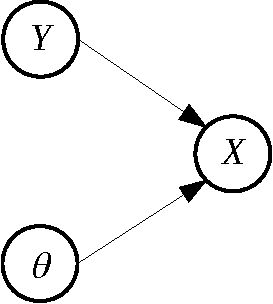
\includegraphics[width=.25\textwidth]{discriminative.pdf}\label{fig:discriminative}}
\caption{Bayesian networks representing generative and discriminative models, where $X$, $Y$ and $\theta$ respectively denote the variable of interest, the data, and the model parameters. Note the marginal independence of~$Y$ and~$\theta$ in the discriminative model.}
\label{fig:graph_comparison}
\end{center}
\end{figure}

Composite likelihood (CL, see \cite{Varin-11} and the references therein) is a semi-generative approach to statistical inference that extends the familiar notion of likelihood without requiring a full generative model. The key idea is to model an arbitrary set of low-dimensional features separately and then combine them, instead of modeling the data distribution as a whole. This may be viewed as a {\em divide and conquer} method to approximate the true but intractable likelihood. While maximum CL does not inherit the general property of maximum likelihood to yield an asymptotically minimum-variance estimator, it is consistent under mild conditions \cite{Xu-11} and may offer an excellent trade-off between computational and statistical efficiency in practice. 

In this note, CL is interpreted as a probabilistic opinion pool of ``agents'' making use of different pieces of information, or clues, extracted from the input data. Each agent acts as an isolated generative model-based statistician and expresses an opinion based on a single clue in the form of a likelihood function of the hidden variables. The agent opinions are then aggregated into a probability distribution on the hidden variables analogous to a Bayesian posterior.

We further argue that a particular log-linear opinion pool yields the best possible predictive distribution in the sense of maximum relative conditional entropy. This perspective entails a method to optimize the weights of the different agents from training data as in a typical discriminative learning scenario. 

%Something for true statisticians. Maybe we could clarify that we use the term ``Bayesian'' in the sense of ``empirical Bayesian'', implying that the parameters $\theta$ are to be estimated somehow contrary to a ``full Bayesian'' approach where they would be integrated out at inference time.


\section{Composite likelihood as opinion pooling}
\label{sec:pool}

Let $Y$ an observable multivariate random variable with sampling distribution $p(y|x)$ conditional on some unobserved variable of interest, $X\in{\cal X}$, where ${\cal X}$ is a known set. Given an experimental outcome $y$, the likelihood is the sampling distribution evaluated at $y$, seen as a function of $x$:
$$
L(x) = p(y|x)
.
$$

This requires a plausible generative model which, for complex data, may be out of reach or involve too many parameters to be estimated. A natural workaround known as {\em data reduction} is to extract some lower-dimensional representation $z=f(y)$, where $f$ is a many-to-one mapping, and consider the potentially more convenient likelihood function:
$$
\ell(x) = p(z|x)
.
$$

Substituting $L(x)$ with $\ell(x)$ boils down to restricting the sample space, thereby  ``delegating'' statistical inference to an ``agent'' provided with partial information. While it is valid for such an agent observing~$z$ only to consider $\ell(x)$ as the likelihood function of the problem, the drawback is that $\ell(x)$ might yield too vague a prediction of~$X$ due to the information loss incurred by data reduction. To make the trick statistically more efficient, we may extract several features, $z_i=f_i(y)$ for $i=1,2,\ldots,n$, and try to combine the likelihood functions $\ell_i(x) = p(z_i|x)$ that they elicit.

If we see the likelihoods as posterior distributions corresponding to uniform priors, this is a classical problem of probabilistic opinion aggregation from possibly redundant sources, for which several methods exist in the literature \cite{Tarantola-82,Genest-86,Garg-04,Allard-12}. We will show in Section~\ref{sec:maxent} that one that is particularly well-suited to our case is the {\em log-linear opinion pool}: 
\begin{equation}
\label{eq:log_pool}
p_\lambda(x|y) = \frac{1}{z_\lambda(y)} \pi(x) \prod_{i=1}^n p(z_i|x)^{\lambda_i},
\end{equation} 
where $\pi(x)$ is some reference distribution or prior, and $\lambda=(\lambda_1,\ldots,\lambda_n)$ is a vector of weights so that the normalizing factor:
$$
z_\lambda(y) = \int \pi(x) \prod_{i=1}^n p(z_i|x)^{\lambda_i} dx
$$
is finite, which holds whenever $\lambda\succeq 0$, {\em i.e.} all weights are positive, assuming that the agent opinions are always upper bounded. Negative weights should be ruled out as the existence condition $z_\lambda(y)<\infty$ would then depend on the particular opinions expressed by the agents. Also note that, while it is possible to have the weights depend on~$y$, there is a strong rational for constant weights as we shall see in the sequel. 

%Strictly positive weights guarantee the so-called 0/1 forcing property, that is, if an hypothesis~$x$ has zero likelihood according to at least one agent, then its consensus probability vanishes too.

% Not clear yet as to what a negative weight could mean!

The log-linear pool~(\ref{eq:log_pool}) bears a striking similarity to Bayes rule, yielding the form: $p_\lambda(x|y)\propto \pi(x) L^c_\lambda(x)$, where the quantity:
\begin{equation}
\label{eq:comp_lik}
L^c_\lambda(x) \equiv \prod_{i=1}^n \ell_i (x)^{\lambda_i}
\end{equation} 
plays the same role as a traditional likelihood function. This expression happens to be known in statistics as a {\em marginal composite likelihood} \cite{Varin-11}. See Appendix~\ref{sec:conditional} for the slightly more general form called {\em conditional composite likelihood}, which can be derived in the same way.

From~(\ref{eq:comp_lik}), we see that CL shares a convenient factorized form with the likelihood derived under the assumption of mutual feature independence, usually referred to as {\em na\"ive Bayes} or {\em simple Bayes} in the machine learning literature, which corresponds to the special case of unitary weights, $\lambda_1=\ldots=\lambda_n= 1$. The clear computational advantage of CL over the true likelihood is that it only requires to evaluate the marginal feature distributions rather than the joint distribution of all features.


\section{Tuning composite likelihood weights}

When the features can be considered exchangeable, it is natural to choose uniform CL weights. The CL is then a scaled version of the na\"ive Bayes likelihood, the common weight value being irrelevant to the maximum CL estimator (MCLE). The weight may be tuned so as to best adjust the pseudo posterior variance matrix to the asymptotic variance matrix of the MCLE \cite{Pauli-11}, or via a close-in-spirit curvature adjustment \cite{Ribatet-12}, in attempts to match the frequentist and composite Bayesian notions of uncertainty.

Ignoring such a goal, another frequent recommandation for CL weights is to sum up to one. This can be motivated in various ways. It turns out that the only pooling operator that does not explicitly depend on~$x$ and preserves {\em external Bayesianity} is the log-linear opinion pool with unit sum weights \cite{Genest-86b}. External Bayesianity essentially means that it should not matter whether the prior is incorporated before or after pooling, provided that all agents agree on the same prior. Another appealing property of log-linear pooling with unit sum weights is to minimize the average Kullback-Leibler (KL) divergence to the agent opinions \cite{Garg-04}. A maximum relative entropy property is also given in \cite{Wang-14}, Theorem~3.

Unit sum weights, however, correspond to the extreme situation where the features are assumed to be maximally redundant, but is clearly ineffective for independent or weakly correlated features, which require weights close to one for the CL to closely approximate the true likelihood. In this case, the CL may be much flatter than it should, leading to severly overestimated credibility sets.

{\color{red} Why is it important to fine-tune the weights?}
We therefore need a method to tune weights that can automatically adjust to the level of statistical dependence beween features.

%Instead, redundancy between agents is assumed by default, and is effectively encoded by the unit sum constraint on weights\footnote{Nevertheless, features which are {\em known} to be mutually independent can be merged into a single feature. This results in increasing their weights in the log-linear pool.}.

\section{Maxent composite likelihood}
\label{sec:maxent}

We can derive composite likelihood from the conditional maximum entropy principle \cite{BergerA-96}. It comes with a method of tuning weights, hence a particular composite likelihood function that we call maxent composite likelihood (MCL).

A cheap MaxEnt argument was already given by \cite{Wang-14}  (standard, non-conditional MaxEnt at fixed $y$, hence just an existence result but no feasible weight tuning).

What we do here is maximum {\em conditional} entropy. It's slightly more complex than a simple $I$-projection. The search space is a set of predictive distributions compatible with mean log-likelihood contraints. If I know the generative distribution, I know the expected log-likelihood.

We work with inequality constraints to force $\lambda\geq 0$:
$$
E[\log p(z_i|x)] \geq c_i \equiv \int \pi(x)p(z_i|x) \log p(z_i|x) dx dy
$$

What does the constraint mean? It means that a model is admissible if it compresses the data at least as well as all my agents. So we are not assuming that the generative models are {\em true}. We only assume that they are useful to compress the (reduced) data. Connection to MDL. 

Why not using the feature-based posteriors or Bayes factors rather than the likelihoods? It's a possibility (perhaps a connection here with Gr\"unwald's luckiness). A justification for not doing it is that the coordinator should discard the priors used by the agents. The constraints are not purely evidence-based since the moments depend on the coordinator's prior but it is arguable a mess of priors wouldn't be good.

Intuition behind weights: Lagrange multipliers to enforce a constraint... Notion of feature relevance. But does $\lambda_1>\lambda_2$ imply that $z_1$ is more relevant than $z_2$? 

The derivation assumed the marginal distribution of the data $h(y)$ to be known. In practice, it is estimated by the empirical distribution just like the moments are estimated.

Game theoretic interpretation \cite{Grunwald-04}.

The dual function boils down to the famous cross-entropy.

Single feature case ($y=z$): the maxent solution has the form $p(x|y)\propto\pi(x)p(y|x)^\lambda$. We expect to have $\lambda=1$ but it's not necessarily the case. It is if $h(y)=\int\pi(x)p(y|x)dx$ because then $h(y)p(x|y)=\pi(x)p(y|x)$ so the constraint is verified (and active). This also tells us that the data marginal should be consistent with the prior on labels for this much expected consistency property to hold. So, either weight datapoints so as to match a desired prior (e.g., uniform) or take the empirical distribution of labels as the ``prior''. 

Which brings another question: in this case, the (unique) weight is insensitive to the prior -- is it true in general? The answer is no. The weights generally depend on the prior. Hence the maxent composite likelihood is prior-dependent. This is an important conceptual difference with the classical notion of likelihood.

\section{Super composite likelihood}
\label{sec:super}

When chosen for computational simplicity, clues may not only convey limited information at individual level: their informativeness may also be very much hypothesis-dependent. Consider, for instance, diagnosing a disease from a routine medical checkup. Body temperature may point to a bacterial infection by comparison with normality, but would not help detecting a non-infectious cardiovascular disease -- and conversely for, say, blood pressure.

This motivates a more general setting where clues can be weighted differently depending on hypotheses.

What happens if we use mean-values constraints conditional on $x$ instead of jointly averaged over $x$ and $y$? This boils down to picking functions of the form:
$$
\chi(x-a)\ell_i(x,y)
$$

The answer is that the maxent solution has the form:
$$
p_\lambda(x|y) = \pi(x) \prod_i p(z_i|x)^{\lambda_i(x)}
$$

In other words, the weights become dependent on the variable of interest. This is the super composite likelihood idea.


\section{Composite EM algorithm for unsupervised learning}
\label{sec:gem}

In a nutshell: alternate unsupervised learning of partial model parameters ($M$-step) and re-estimation of label posteriors via maxent ($E$-step). 

$M$-step: given a posterior estimate $q(x|y)$, do just as if the features were independent and solve: 
$$
\max_\theta
\int \sum_i h(y)q(x|y) \log p_\theta(z_i,x) dx dy
$$

Note we can estimate cross-feature parameters such as class proportions.

Surrogate $E$-step: given generative parameters, recompute the moment constraints and update $q(x|y)$ according to the conditional maxent principle:
$$
\min_q
\int h(y)q(x|y) \log \frac{q(x|y)}{\pi(x)} dx dy
$$
s.t.
$$
\int h(y)q(x|y)\log p_\theta(z_i|x) dx dy \geq \int \pi(x)p_\theta(z_i|x)\log p_\theta(z_i|x) dx dy
$$

However, there is an important issue: how is $h(y)$ defined in both the $M$- and $E$-steps? In supervised context, $h(x,y)$ can be defined beforehand as the prior-corrected empirical distribution:
$$
h(x,y) = \pi(x) \frac{h_0(x,y)}{h_0(x)},
$$
where $h_0(x,y)$ is the raw empirical distribution. In unsupervised context, the best we can do is to replace $h_0(x,y)$ with $h_0(y)q(x|y)$, implying that the empirical distribution of $y$ is reweighted according to:
$$
h(y) = \sum_i w_i\delta(y-y_i),
\qquad
w_i = \int \pi(x)\frac{q(x|y_i)}{\sum_j q(x|y_j)} dx,
$$
which needs to be done each time $q(x|y)$ is updated, that is, after each $E$-step.

The other option is to keep $h(y)$ constant throughout the iterations but adapt $\pi(x)$ as the marginal distribution of labels learned in the $M$-step. In this case, it's no longer a ``prior''. 

Are we minimizing a unique functional as in the variational EM algorithm? Possibly not. We may see this generalization as a two-player game. One player tries to predict several data features independently. The other player tries to predict labels. Together, they find patterns (clusters) in unlabeled data. Does the more general version converge? Does the game have a value? And so on.

In the case of a single feature, is this the well-known EM? The $M$-step is clearly the same, what about the $E$-step? It is the same if $h(y)p_\theta(x|y)=p_\theta(y|x)\pi(x)$. However, this condition won't hold if $h(y)$ is an empirical distribution... In this special case, the ``E player'' could use the data distribution model produced by the ``M player'' instead of the empirical one but, more generally, there is no data distribution model so he has to stick to the empirical one.

The maxent is a surrogate for the $E$-step. It reflects the lack of a full model $p_\theta(x,y)$.

% Accounting here for Xi'An comment on xianblog.wordpress.com
% The sum of the powers is constrained to be equal to one, even though
% I do not understand why the dimensions of the projections play nog
% role in this constraint. Simplicity is advanced as an argument,
% which sounds rather weak…
%This simple constraint is implied by the external Bayesianity requirement: as it turns out, the only aggregation operator which is both externally Bayesian and independent from $x$ boils down to plugging a composite likelihood with unit sum weights into Bayes rule, hence extending the classical notion of likelihood in Bayesian analysis.


\section{Discussion}
\label{sec:discussion}

Deep learning is discriminative...

CL is a concept from computational statistics that has mainly been developed so far in a frequentist perspective as a surrogate for the maximum likelihood method. We have shown a deep connection between CL and probabilistic inference, thereby establishing CL as a class of discriminative models. Because CL is built from a set of marginal feature-specific generative distributions, it is in essence a two-step semi-generative, semi-discriminative learning approach. In the first, ``generative'' phase, the feature distributions are learned; in the second, ``discriminative'' phase, the feature weights are learned. This strategy can be thought of as a form of non-adaptive boosting.

%The first phase corresponds to the training of ``weak learners''. The second phase amounts to a form of boosting. 

A purely discriminative learning could be used instead but...
Why potentially more efficient than pure discriminative training: because generative training is always more efficient than discriminative training if models are comparable. So the key point is that ``we have less parameters in the discriminant phase". Good in small datasets. But also in asymptotic regime if the features are weakly or highly correlated (???).

Logistic regression / naive Bayes example. Under homoscedasticity (assuming that each feature has class-independent variance), CBI is equivalent to logistic regression -- because the predictive distribution family is the same. This is a case where BCI brings nothing. But consider heteroscedasticity, then BCI yields a quadratic classifier. Compared to a fully discriminative model, the number of parameters to learned in the discriminative phase is reduced by half.

The first training phase is easier if supervised but could be unsupervised too (using mixture models). How do we then deal with label switching issues? Can we safely assume conditional feature independence {\em in the generative training phase}? I believe so provided that the marginal distribution parameters are disjoint. It's obvious in the supervised learning scenario.

If unsupervised, the first learning phase could be compared with contrastive pre-training of RBMs \cite{Hinton-06,Fischer-14}, which also optimize parameters for generation of observable features. BCI is comparable with an RBM with a single output unit (which is just a generative model assuming conditionial feature independence). The key difference is that the RBM is a full generative model while BCI only deals with marginal models, hence relying on weaker assumptions. This won't change anything in the pre-training phase but RBMs have to deal with more parameters in the generative learning phase. In fully supervised context, RBM pre-training is pointless since all parameters learned in the first phase will be overwritten. In BCI, pre-training is crucial even in supervised context because the parameters learned in the discriminative phase (the feature weighs) describe a sub-manifold of the predictive distribution family.

Needs features. Not a representation learning method, but could be coupled why not.


%{\color{red} Moreover, while RBM parameters are typically refined in a supervised discriminative learning step, disjoint set of parameters for SCL. Dunno how to say that.} 

%In such context, SCL competes with classical discriminative models (logistic regression, Gaussian processes \cite{Rasmussen-06}, maximum entropy models \cite{BergerA-96}, etc.), and may compare more or less favorably in practice depending on the amount of training data. For relatively small training datasets, we may hope for more accurate inference using~SCL than using traditional discriminative models, extrapolating from the results of \cite{Ng-01} regarding the comparison between logistic regression and na\"ive Bayes classifiers.
%{\color{red}Ici, il manque la comparaison avec les RBMs qui ne sont pas (forcement) des modeles discriminatifs.}

%%, hence alleviating the need for heavily supervised model training

%In summary, CL has the potential to yield weakly supervised or unsupervised Bayesian-like inference procedures depending on the particular task at hand. This property reflects the encoding of statistical relationships between the data and {\em all} unknown parameters. CL thus appears as a trade-off between generative models, which are optimal for unsupervised learning but possibly intractable, and traditional discriminative models (logistic regression, Gaussian processes \cite{Rasmussen-06}, maximum entropy models \cite{BergerA-96}, etc.), which are inherently supervised. CL models are discriminative models assembled from atomic generative models and, from this point of view, may be considered as {\em semi-generative} models.

%CL may be considered as a {\em semi-generative} model: a discriminative model assembled from partial generative models.

%As a note of caution, we shall stress that the pre-determined weights assigned to the different associations between observed and unobserved values represent prior knowledge regarding the informativeness of clues. A poor choice of weights will inevitably result in a poor approximation to the ``true'' Bayesian posterior -- the posterior that would be obtained from a realistic generative model if it was tractable. In future work, we will investigate feature selection strategies to mitigate this problem.

% Improve the discussion on following aspects:
% ** Why is it compatible with unsupervised learning? Give more insight.
% ** Stress the contribution: class-specific weighting.
% * Pivotality argument.
% * Bayes is a special case of composite Bayes.

{\color{red}Product of fucking experts \cite{Hinton-02}. Log-linear pool to build a generative model (assuming in fact independence between experts). Better seen as a ``log-mixture model''. Sounds like each expert is associated with a class, so it's the same as a RBM. Contrastive learning approximates ML parameter estimation. The experts are learning jointly. It's just a generative model.}

{\color{red}Two-step training: generative phase then discriminative phase. Why is it cool?}

{\color{red}CBI is just a way to reweight Naive Bayes. What's the big deal? Can we really expect massively superior performance? Are we just talking about realistic credibility sets?}


\appendix

\section{Conditional composite likelihood}
\label{sec:conditional}

As a straightforward  extension of marginal CL, each feature-based likelihood may be conditioned by an additional ``independent'' feature $z^c_i = f^c_i(y)$ considered as a predictor of the ``dependent'' feature, $z_i=f_i(y)$, yielding the more general form:
\begin{equation}
\label{eq:cond_feat_lik}
\ell_i(x) = p(z_i|x,z^c_i).
\end{equation}

Conditioning may be useful if it is believed that $z^c_i$ alone is little or not informative about $x$, but can provide relevant information when considered jointly with $x$, as in the case of regression covariates, for instance. Equation~(\ref{eq:comp_lik}) then amounts to conditional CL \cite{Varin-11}, a more general form of CL also including Besag's historical {\em pseudo-likelihood} \cite{Besag-74} developed for image segmentation.


\section{Minimally discriminative model}

Let $\pi(x)$ some reference distribution that represents full
uncertainty about $X$. We wish to select the joint distribution
$p(x,y)$ that minimizes:
$$
I(p) = \int p(x,y) \log \frac{p(x|y)}{\pi(x)} dy,
$$ subject to feature mean-value constraints of the form:
$$
\int p(x,y) f(x,y) dx dy = \mu.
$$

There are two special cases of this problem in the literature.  On the
one hand, the {\em maximum entropy classifier} \cite{BergerA-96}
incorporates the constraint that $p(y)$ be known, however we will see
that this is not necessary. The {\em minimally informative likelihood}
method \cite{Yuan-99b,Yuan-99}, on the other hand, imposes that
$p(x)=\pi(x)$, hence assuming the form $p(x,y)=\pi(x)p(y|x)$. We won't
make such assumptions here and will consider the case where $\mu$ is
completely unknown.

The above problem is seen to be equivalent to minimizing the auxiliary
objective function:
$$
I(p,m) 
= \int p(x,y) \log \frac{p(x,y)}{\pi(x)m(y)} dxdy,
$$ over $p$ and $m$, subject to the same constraints on $p$. We note
that $I(p,m)=I(p)+D(p_y\|m)$, showing that the auxiliary function
essentially adds a penalty term to the actual objective in order to
force $p(y)$ close to $m(y)$.

Minimizing $I(p,m)$ along both $p$ and $m$ is basically a minimum KL
divergence problem between two convex distribution spaces, so there
must be a unique solution {\bf -- to be checked in
  \cite{Cover-91}}. It is similar to the rate-distortion problem in
information theory, which may be solved by alternate minimization,
yielding a Blahut-Arimoto algorithm.
\begin{itemize}
\item {\em Let's call it A-step}. Optimize $p(x,y)$ at fixed $m$
  s.t. constraint:
$$
\exists \lambda, \qquad
p_{\lambda,m}(x,y) = \frac{1}{Z(\lambda, m)} \pi(x) m(y) e^{-\lambda^\top t(x,y)}
$$
The actual $\lambda$ is found my maximizing the dual function
$\psi(\lambda,m)$, see below.
\item {\em Let's call it B-step}. Optimize $m(y)$ at fixed $p(x,y)$:
$$
m(y) = \int p(x,y) dx
$$
\end{itemize}

Upon convergence, the algorithm outputs both joint and marginal
distributions $p_{\star}(x,y)$ and $m_{\star}(y)$ that both depend on
$\mu$. By construction, we have that $p_{\star}(y) = m_{\star}(y)$,
therefore $p_\star(x|y)=p_{\star}(x,y)/m_{\star}(y)$.


\section{Comparison with maximum entropy classifier}

Lagrangian...
$$
{\cal L}(p,m,\lambda)
= 
\int p(x,y) \log \frac{p(x,y)}{\pi(x)m(y)} dxdy
+
\lambda^\top \left( 
\int p(x,y) f(x,y) dydy - \mu 
\right)
$$ where $\lambda$ represents a vector-valued Lagrange multiplier. At
fixed $m$, the solution has the form:
$$
p_{\lambda,m}(x,y) = \frac{1}{Z(\lambda,m)}
\pi(x) m(y) e^{-\lambda^\top f(x,y)} 
$$

Note that this implies that the conditional distribution is
independent of $m$ once $\lambda$ is determined,
$$
p_\lambda(x|y) = \frac{1}{z(\lambda,y)} \pi(x) e^{-\lambda^\top f(x,y)} 
$$

Also, the marginal is a modulation of $m(y)$:
$$
p_{\lambda,m}(y) = \frac{z(\lambda,y)}{Z(\lambda,m)} m(y)
$$

Dual function at fixed $m$:
$$
\psi(\lambda,m) 
\equiv \min_p {\cal L}(p,m,\lambda)
= 
- \log Z(\lambda,m) - \lambda^\top \mu
.
$$ 

An alternative expression is:
$$
\psi(\lambda, m)
= 
\int h(x,y) 
\log \frac{p_{\lambda,m}(x,y)}{\pi(x)m(y)} dxdy,
$$ where $h(x,y)$ is any distribution statisfying the
constraints. This shows that maximizing the dual function at fixed $m$
is essentially the same as minimizing the KL divergence
$D(h\|p_{\lambda,m})$ over $\lambda$, in other words fitting $h(x,y)$
by some distribution of the form $p_{\lambda,m}$. The fact that the
result does not depend on the particular $h(x,y)$ that is chosen, as
long as it satifies the constraint, is a general property of
exponential families.

We also have that the dual function associated with $I(p)$ reads:
\begin{eqnarray*}
\psi(\lambda) 
 & = & \min_m \psi(\lambda, m)\\
 & = & \int h(x,y) \log \frac{p_{\lambda}(x|y)}{\pi(x)} dxdy\\
 & = & -\int h(y) \log z(\lambda,y) dy - \lambda^\top \mu
\end{eqnarray*}

But, wait, that's exactly what we get in the maximum entropy
classifier! So, at the end of the day, we simply got an alternative
method to learn $\lambda$ in the maximum entropy classifier, i.e. the
Blahut-Arimoto algorithm as opposed to a brute-force maximization of
$\psi(\lambda)$. Both methods will converge to the same $\lambda$...

What it essentially means is that the optimal $\lambda$ is insensitive
to $m(y)$ as long as $m(y)$ is compliant in the sense that:
$$
m(y) = \int h(x,y) dx,
$$ for some distribution $h(x,y)$ statisfying the constraint. This is
true for the optimal $m_\star(y)$ output by the BA algorithm, but
also, for instance, for the empirical distribution of observations in
a training dataset used to estimate $\mu$, as proposed in
\cite{BergerA-96}. The only special property of $m_\star(y)$ is to
yield the full Bayesian model $p_\star(x,y)=p_\star(x|y)m_\star(y)$
that minimizes the discrimination information. We may not care too
much about that in practice since we will only use $p_\star(x|y)$. 

\section{Comparison with minimally informative likelihood}

Yuan \cite{Yuan-99} considered the situation where we add the
constraint that $p(x)=\pi(x)$ to the minimum discrimination inference
problem. Unknown is then the conditional distribution
$p(y|x)$. Lagrangian...
\begin{eqnarray*}
{\cal L}(p,m,\lambda)
 & = & 
\int \pi(x)p(y|x) \log \frac{p(y|x)}{m(y)} dxdy
+
\lambda^\top \left( 
\int \pi(x)p(y|x) f(x,y) dydy - \mu 
\right) \\
 & = & 
\int \pi(x)
\left( 
\int
p(y|x) \log \frac{p(y|x)}{m(y)} dy
+
\lambda^\top 
\int p(y|x) f(x,y) dy
- \mu 
\right)
dx 
\end{eqnarray*}

The derivative is given by,
$$
\frac{\partial\cal L}{\partial p(y|x)}
= 
\pi(x)\left[ 
1 + \log \frac{p(y|x)}{m(y)} 
+ \lambda^\top f(x,y)
\right],
$$
hence the optimal model at fixed $m$ has the form:
$$
p_{\lambda,m}(y|x) = \frac{1}{Z(\lambda,m,x)} m(y) e^{-\lambda^\top f(x,y)} 
$$

Note that the induced posterior distribution $p_{\lambda,m}(x|y)$ has
a different form from above unless the normalizing factor
$Z(\lambda,m,x)$ turns out independent from $x$. If this is not the
case, we no longer have the property that $p_{\lambda,m}(x|y)$ is
independent from $m$ given $\lambda$.

Dual function...
$$
\psi(\lambda,m) 
=
- \int \pi(x) \log Z(\lambda, m, x) dx
- \lambda^\top \mu
$$

Equivalently, for any distribution under the form $\pi(x)h(y|x)$ that
satisfies the moment constraint, we have:
$$
\psi(\lambda,m) 
=
\int \pi(x) h(y|x) \log \frac{p_{\lambda,m}(y|x)}{m(y)} dxdy
$$

Now, the real question is why should we constrain $p(x)$, which boils
down to a Bayesian prior in this context, to be the same as our
reference $\pi(x)$? It only makes sense if we want our inference to
stick to a generative modeling paradigm... but haven't we already
given up on that? Therefore, unless we find a good reason not to, we
won't impose the $p(x)=\pi(x)$ constraint, thereby allowing for a
discrepancy between the reference and the prior.


\section{Discriminative vs. semi-discriminative}

Let's go back to the equivalence we found between our approach and the
maximum entropy classifier (MCE) \cite{BergerA-96}. We have said that
the former is essentially a re-formulation of MCE.

But the re-formulation also conveys a generalization of MCE if,
instead of letting $m$ being an arbitrary distribution, we restrict
its search space to some set of acceptable reference
distributions. Would such a strategy be useful? 

Recall that the method selects the joint distribution that minimizes
discriminative information, as defined by $I(p)$:
$$
I(p) 
= \int p(x,y)\log\frac{p(x|y)}{\pi(x)} dxdy
= E_Y[D(p_{x|y}\|\pi)]
$$

The latter characterization reminds us that discriminative information
is defined in an average sense. The corresponding posterior $p(x|y)$
may not be conservative for some $y$, in particular those that are
unlikely under $p(y)$. It would be a problem if that's the case for
the particular data at hand. For that to happen rarely, the ideal
$p(y)$ would be the ``true'' marginal distribution of $Y$.

However, for vague mean value constraints, nothing may prevent the
optimal $m_\star(y)$ from departing significantly from that ideal
distribution. In fact, we can show that $m_\star(y)$ only has mass at
$y$ values that maximize $z(\lambda_\star,y)$, and is therefore likely
sparse. This is because $m_\star$ minimizes $\psi(\lambda_\star,m)$,
which is equivalent to maximizing $Z(\lambda_\star,m)$ and we have:
$$
Z(\lambda, m) = \int m(y) z(\lambda, y) dy.
$$

In other words, the solution to our problem may be singular! It does
not hurt since, as discussed above, one may alternatively fix $m(y)$
to some pre-defined distribution... but this, in practice, restricts
the method to supervised learning situations.

We may not face this issue with the MIL method, which further imposes
the prior on $X$, so all the information from the constraints goes
into specifying a possibly reasonable generative model.



\bibliographystyle{abbrv}
\bibliography{cvis,stat,alexis}

%%\input{draft.biblio}

\end{document}


\end{document}


\end{document}


\end{document}
